\documentclass[11pt,letterpaper]{report}
\usepackage[utf8]{inputenc}
\usepackage[T1]{fontenc}
\usepackage{geometry}
\usepackage{graphicx}
\usepackage{hyperref}
\usepackage{listings}
\usepackage{xcolor}
\usepackage{fancyhdr}
\usepackage{tocloft}
\usepackage{titlesec}
\usepackage{booktabs}
\usepackage{longtable}
\usepackage{multirow}
\usepackage{amsmath}
\usepackage{bytefield}
\usepackage{tikz}
\usetikzlibrary{shapes.geometric, arrows.meta, positioning, fit, backgrounds, calc}
\usepackage{varwidth} % Add to preamble
% Page geometry
\geometry{margin=1in}

% List formatting (compact for NSF page limits)
\usepackage{enumitem}
\setlist[itemize]{nosep}
\setlist[enumerate]{nosep}
\setlist[description]{nosep}

% Hyperref setup
\hypersetup{
    colorlinks=true,
    linkcolor=blue,
    filecolor=magenta,      
    urlcolor=cyan,
    pdftitle={VGA Graphics Controller User Manual},
    pdfauthor={Larry D. Pyeatt},
}

% Code listing style
\lstdefinestyle{vhdl}{
    language=VHDL,
    basicstyle=\ttfamily\small,
    keywordstyle=\color{blue}\bfseries,
    commentstyle=\color{green!60!black},
    stringstyle=\color{red},
    numbers=left,
    numberstyle=\tiny\color{gray},
    stepnumber=1,
    numbersep=8pt,
    backgroundcolor=\color{gray!10},
    showspaces=false,
    showstringspaces=false,
    showtabs=false,
    frame=single,
    tabsize=2,
    captionpos=b,
    breaklines=true,
    breakatwhitespace=false,
}

\lstdefinestyle{c}{
    language=C,
    basicstyle=\ttfamily\small,
    keywordstyle=\color{blue}\bfseries,
    commentstyle=\color{green!60!black},
    stringstyle=\color{red},
    numbers=left,
    numberstyle=\tiny\color{gray},
    stepnumber=1,
    numbersep=8pt,
    backgroundcolor=\color{gray!10},
    showspaces=false,
    showstringspaces=false,
    showtabs=false,
    frame=single,
    tabsize=4,
    captionpos=b,
    breaklines=true,
    breakatwhitespace=false,
}

% Header and footer
\pagestyle{fancy}
\fancyhf{}
\fancyhead[L]{\leftmark}
\fancyhead[R]{VGA Graphics Controller}
\fancyfoot[C]{\thepage}

% Title formatting
\titleformat{\chapter}[display]
{\normalfont\huge\bfseries}{\chaptertitlename\ \thechapter}{20pt}{\Huge}
\titlespacing*{\chapter}{0pt}{-50pt}{40pt}

\begin{document}

% Title page
\begin{titlepage}
    \centering
    \vspace*{2cm}
    
    {\Huge\bfseries VGA Graphics Controller\\[0.5cm]}
    {\LARGE User Manual\\[2cm]}
    
    {\Large Hardware IP Core for Xilinx FPGAs\\[1cm]}
    
    \vfill
    
    {\large\textbf{Larry D. Pyeatt}\\[1cm]}
    
    {\large Version 1.0\\[0.5cm]}
    {\large \today\\[2cm]}
    
    \vfill
    
    {\large Dual-Resolution Display Controller\\
    with Double-Buffering and Palette Support\\[2cm]}
    
    \vfill
    
    {\footnotesize Copyright \copyright\ 2026 Larry D. Pyeatt\\
    All rights reserved.}
    
\end{titlepage}

% Table of contents
\tableofcontents
\listoftables
\listoffigures

% Chapters
\chapter{Introduction}

\section{About This Manual}

This manual provides complete documentation for the VGA Graphics Controller, a dual-resolution display controller designed for Xilinx Field-Programmable Gate Arrays (FPGAs). This hardware IP core enables you to generate standard VGA video signals for connecting to monitors and displays.

Whether you're building a retro gaming console, creating custom graphics applications, developing embedded systems with display capabilities, or learning about digital display systems, this manual will guide you through every aspect of the VGA Graphics Controller.

\section{What is the VGA Graphics Controller?}

The VGA Graphics Controller is a synthesizable VHDL IP core that generates industry-standard VGA timing signals and manages framebuffer memory. It provides a complete solution for adding graphics capabilities to your FPGA design.

\subsection{Key Features}

\begin{itemize}
    \item \textbf{Dual Resolution Modes:}
    \begin{itemize}
        \item 320$\times$200 pixels with 2$\times$2 pixel doubling (displayed as 640$\times$400)
        \item 640$\times$400 pixels native resolution
    \end{itemize}
    
    \item \textbf{Color Support:}
    \begin{itemize}
        \item 8-bit indexed color (256 simultaneous colors)
        \item 12-bit RGB palette (4,096 possible colors: R4G4B4)
        \item Programmable color lookup table (palette)
    \end{itemize}
    
    \item \textbf{Memory Architecture:}
    \begin{itemize}
        \item Internal framebuffer using FPGA Block RAM
        \item 256 KB total framebuffer memory
        \item Dual-port architecture for simultaneous CPU and display access
        \item Double-buffering support in 320$\times$200 mode
    \end{itemize}
    
    \item \textbf{Interface:}
    \begin{itemize}
        \item AXI4-Lite slave interface for CPU access
        \item Memory-mapped framebuffer and palette
        \item Simple register-based control
    \end{itemize}
    
    \item \textbf{Display Specifications:}
    \begin{itemize}
        \item 640$\times$400 @ 70 Hz output
        \item 25.175 MHz pixel clock
        \item Standard VGA timing (VESA compatible)
        \item Separate H-SYNC and V-SYNC outputs
        \item 12-bit digital RGB output (4 bits per channel)
    \end{itemize}
\end{itemize}

\subsection{Target Applications}

This VGA controller is ideal for:

\begin{itemize}
    \item Retro gaming systems and consoles
    \item Embedded systems with display requirements
    \item Educational projects for learning computer graphics
    \item Industrial control panels and HMI systems
    \item FPGA-based soft processors (MicroBlaze, RISC-V, etc.)
    \item Test equipment and diagnostic displays
    \item Digital art and creative coding projects
\end{itemize}

\section{Who Should Read This Manual?}

This manual is intended for engineers, developers, and hobbyists working with:

\begin{itemize}
    \item FPGA development and digital design
    \item Embedded systems programming
    \item Computer graphics and display systems
    \item Retro computing and gaming
    \item Educational projects in computer engineering
\end{itemize}

\section{Prerequisites}

\subsection{Required Knowledge}

To effectively use this VGA controller, you should be familiar with:

\begin{itemize}
    \item FPGA development flow (synthesis, implementation, bitstream generation)
    \item Xilinx Vivado design tools
    \item Basic VHDL (for understanding the design, optional for use)
    \item C programming (for writing software to control the display)
    \item AXI bus protocol basics (helpful but not required)
    \item Basic understanding of raster graphics and frame buffers
\end{itemize}

\subsection{Required Hardware}

Minimum hardware requirements:

\begin{itemize}
    \item Xilinx FPGA development board (Artix-7 or higher recommended)
    \item VGA connector (most dev boards include this)
    \item VGA-capable monitor supporting 640$\times$400 @ 70 Hz
    \item VGA cable
    \item USB cable for FPGA programming
\end{itemize}

\subsection{Required Software}

\begin{itemize}
    \item Xilinx Vivado Design Suite (2018.3 or later)
    \item Text editor or IDE for C programming
    \item (Optional) Xilinx SDK or Vitis for embedded software development
\end{itemize}

\section{Document Conventions}

Throughout this manual, the following conventions are used:

\begin{itemize}
    \item \texttt{Monospace text} indicates code, register names, or memory addresses
    \item \textbf{Bold text} highlights important concepts or warnings
    \item \textit{Italic text} introduces new terminology
    \item Hexadecimal values are prefixed with \texttt{0x}
    \item Binary values are prefixed with \texttt{0b}
\end{itemize}

\chapter{Hardware Overview}

\section{System Architecture}

The VGA Graphics Controller consists of several key hardware blocks that work together to generate video signals and manage graphics memory.

\subsection{Block Diagram}

The complete system architecture is shown in Figure~\ref{fig:block_diagram}.

\begin{figure}[tbp]
\centering
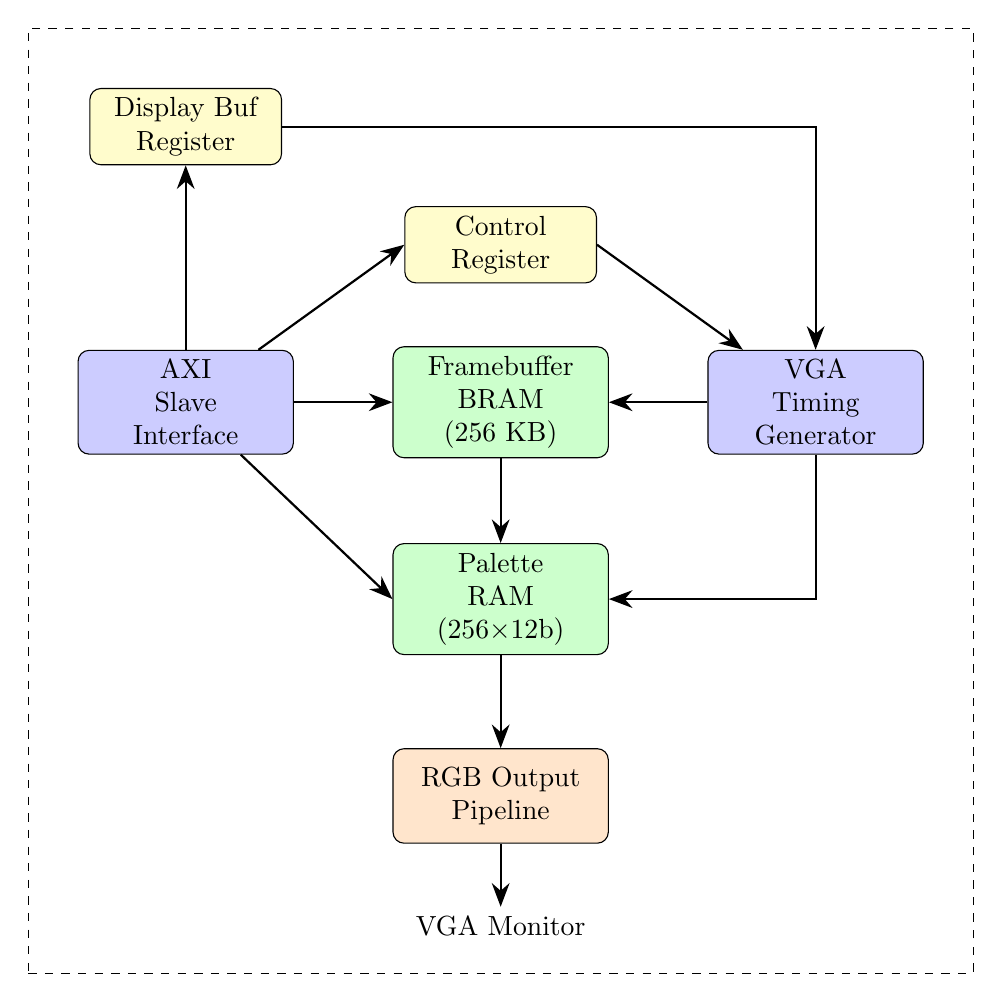
\begin{tikzpicture}[
    block/.style={rectangle, draw, fill=blue!20, text width=2.5cm, text centered, minimum height=1.2cm, rounded corners},
    memory/.style={rectangle, draw, fill=green!20, text width=2.5cm, text centered, minimum height=1.2cm, rounded corners},
    register/.style={rectangle, draw, fill=yellow!20, text width=2.2cm, text centered, minimum height=0.8cm, rounded corners},
    arrow/.style={-{Stealth[length=3mm]}, thick},
    container/.style={rectangle, draw, dashed, inner sep=0.3cm}
]
% Main container
\node[container, minimum width=12cm, minimum height=12cm] (container) at (0,1.25) {};
%\node[above] at (container.north) {\textbf{VGA Controller Top Level}};
% Top row blocks
\node[block] (axi) at (-4, 2.5) {AXI\\Slave\\Interface};
\node[memory] (fb) at (0, 2.5) {Framebuffer\\BRAM\\(256 KB)};
\node[block] (timing) at (4, 2.5) {VGA\\Timing\\Generator};
% Control registers (left side)
\node[register] (ctrl) at (0, 4.5) {Control\\Register};
\node[register] (disp) at (-4, 6) {Display Buf\\Register};
% Middle row
\node[memory] (pal) at (0, 0) {Palette\\RAM\\(256$\times$12b)};
% Bottom
\node[block, fill=orange!20] (pipeline) at (0, -2.5) {RGB Output Pipeline};
% Arrows from AXI to memories
\draw[arrow] (axi.east) -- (fb.west);
\draw[arrow] (axi) -- (pal.west);
% Arrows from AXI to registers
\draw[arrow] (axi) -- (ctrl.west);
\draw[arrow] (axi.north) -- (disp.south);
% Arrows from registers to blocks
\draw[arrow] (ctrl.east) -- (timing);
\draw[arrow] (disp.east) -| (timing.north);
% Arrows for data flow
\draw[arrow] (timing.west) -- (fb.east);
\draw[arrow] (timing.south) |- (pal.east);
\draw[arrow] (fb.south) -- (pal.north);
\draw[arrow] (pal.south) -- (pipeline.north);
% External connections
\node[below=0.8cm of pipeline] (monitor) {VGA Monitor};
\draw[arrow] (pipeline.south) -- (monitor.north);
\end{tikzpicture}
\caption{VGA Controller Block Diagram}
\label{fig:block_diagram}
\end{figure}

\subsection{Component Descriptions}

\subsubsection{VGA Timing Generator}

The timing generator produces all necessary VGA synchronization signals:

\begin{itemize}
    \item Horizontal sync (H-SYNC) pulse
    \item Vertical sync (V-SYNC) pulse
    \item Pixel clock enable signals
    \item Video blanking control
    \item Framebuffer address generation
\end{itemize}

The timing generator operates at 25.175 MHz (the VGA pixel clock) and generates timing for 640$\times$400 @ 70 Hz display mode. It automatically handles pixel doubling when in 320$\times$200 mode.

\subsubsection{Framebuffer BRAM}

The framebuffer is implemented using FPGA Block RAM and stores pixel data:

\begin{itemize}
    \item Total size: 256 KB
    \item Organization: Byte-addressable (8 bits per pixel)
    \item AXI Interface: Supports byte, halfword, and word writes (1, 2, or 4 bytes per transaction)
    \item Dual-port architecture:
    \begin{itemize}
        \item Port A: Connected to AXI interface (CPU read/write)
        \item Port B: Connected to VGA timing generator (display read)
    \end{itemize}
    \item Supports two 320$\times$200 buffers (double-buffering) or one 640$\times$400 buffer
\end{itemize}

\subsubsection{Color Palette RAM}

The palette provides color lookup functionality:

\begin{itemize}
    \item 256 entries (matching 8-bit pixel values)
    \item 12-bit RGB color depth per entry (4 bits per channel)
    \item Dual-port architecture for CPU and display access
    \item Programmable through AXI interface
\end{itemize}

\subsubsection{AXI4-Lite Slave Interface}

Provides CPU access to all controller resources:

\begin{itemize}
    \item Memory-mapped framebuffer access
    \item Palette programming interface
    \item Control and status registers
    \item Standard AXI4-Lite protocol
    \item Low-latency access: 2 AXI cycles (registers/palette), 2-5 cycles (framebuffer multi-byte writes)
\end{itemize}

\subsubsection{RGB Output Pipeline}

Converts indexed pixel data to RGB signals:

\begin{itemize}
    \item Two-stage pipeline for timing closure
    \item Palette lookup operation
    \item Video blanking insertion
    \item 12-bit RGB output (4 bits per channel)
\end{itemize}

\section{Clock Domains}

The VGA controller operates with two independent clock domains, as illustrated in Figure~\ref{fig:clock_domain}.

\begin{figure}[tbp]
\centering
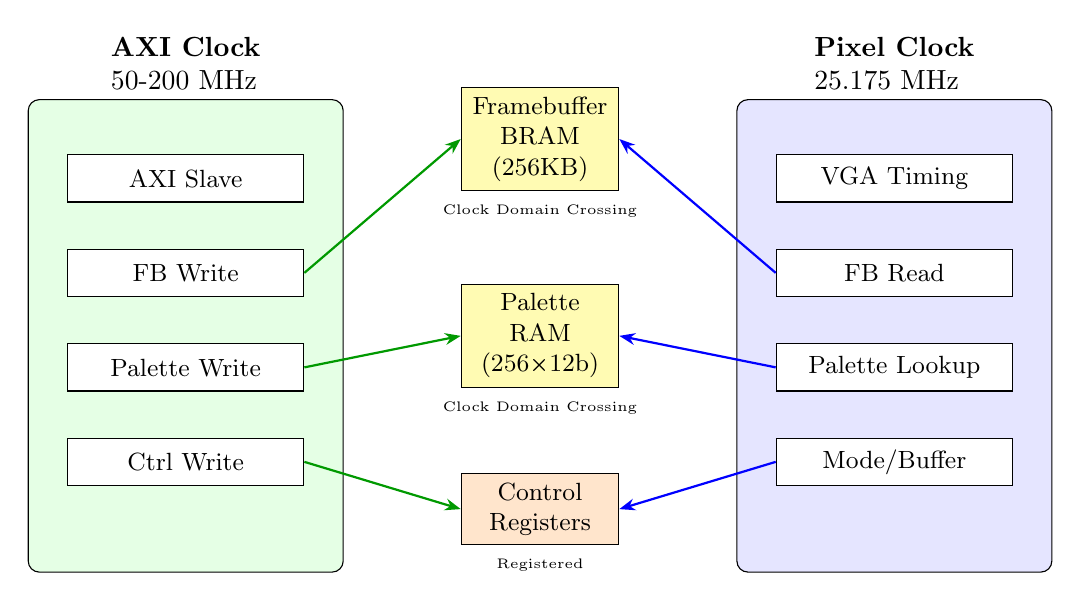
\begin{tikzpicture}[
    clockdomain/.style={rectangle, draw, fill=blue!20, rounded corners, minimum width=4cm, minimum height=6cm, align=center},
    block/.style={rectangle, draw, fill=white, minimum width=3cm, minimum height=0.6cm, font=\small},
    memblock/.style={rectangle, draw, fill=yellow!30, minimum width=2cm, minimum height=0.8cm, font=\small, align=center},
    arrow/.style={-{Stealth[length=2mm]}, thick}
]
% AXI clock domain (LEFT)
\node[clockdomain, fill=green!10] (axi_domain) at (-4.5, 0) {};
\node[above] at (axi_domain.north) {\begin{varwidth}{\textwidth}\textbf{AXI Clock}\\50-200 MHz\end{varwidth}};
\node[block] (axi) at (-4.5, 2) {AXI Slave};
\node[block] (fb_write) at (-4.5, 0.8) {FB Write};
\node[block] (pal_write) at (-4.5, -0.4) {Palette Write};
\node[block] (ctrl_write) at (-4.5, -1.6) {Ctrl Write};

% Pixel clock domain (RIGHT)
\node[clockdomain, fill=blue!10] (pix_domain) at (4.5, 0) {};
\node[above] at (pix_domain.north) {\begin{varwidth}{\textwidth}\textbf{Pixel Clock}\\25.175 MHz\end{varwidth}};
\node[block] (timing) at (4.5, 2) {VGA Timing};
\node[block] (fb_read) at (4.5, 0.8) {FB Read};
\node[block] (pal_read) at (4.5, -0.4) {Palette Lookup};
\node[block] (ctrl_read) at (4.5, -1.6) {Mode/Buffer};

% Memory blocks in middle - MORE VERTICAL SPACING
\node[memblock] (fb_mem) at (0, 2.5) {Framebuffer\\BRAM\\(256KB)};
\node[memblock] (pal_mem) at (0, 0) {Palette\\RAM\\(256×12b)};
\node[memblock, fill=orange!20] (ctrl_reg) at (0, -2.2) {Control\\Registers};

% Arrows - Framebuffer
\draw[arrow, green!60!black] (fb_write.east) -- (fb_mem.west);
\draw[arrow, blue] (fb_read.west) -- (fb_mem.east);

% Arrows - Palette
\draw[arrow, green!60!black] (pal_write.east) -- (pal_mem.west);
\draw[arrow, blue] (pal_read.west) -- (pal_mem.east);

% Arrows - Control registers
\draw[arrow, green!60!black] (ctrl_write.east) -- (ctrl_reg.west);
\draw[arrow, blue] (ctrl_read.west) -- (ctrl_reg.east);

% Clock domain crossing labels
\node[below=0.05cm of fb_mem, font=\tiny] {Clock Domain Crossing};
\node[below=0.05cm of pal_mem, font=\tiny] {Clock Domain Crossing};
\node[below=0.05cm of ctrl_reg, font=\tiny] {Registered};

\end{tikzpicture}
\caption{Clock Domain Architecture}
\label{fig:clock_domain}
\end{figure}

\subsection{Pixel Clock Domain (25.175 MHz)}

\begin{itemize}
    \item VGA timing generation
    \item Framebuffer reads for display
    \item Palette lookups
    \item RGB output pipeline
\end{itemize}

This clock must be generated from your board's oscillator using a clock management primitive (MMCM or PLL). The provided TCL script automatically creates a clocking wizard configured for this frequency.

\subsection{AXI Clock Domain (50-200 MHz)}

\begin{itemize}
    \item AXI4-Lite slave interface
    \item CPU framebuffer writes
    \item Palette updates
    \item Control register access
\end{itemize}

This clock typically comes from your processor or system interconnect. Clock domain crossing is handled automatically by the dual-port Block RAM.

\section{Resource Utilization}

Actual resource usage on Xilinx Artix-7 XC7A100T (post-synthesis):

\begin{table}[tbp]
\centering
\caption{FPGA Resource Utilization}
\label{tab:resources}
\begin{tabular}{lrrr}
\toprule
\textbf{Resource} & \textbf{Used} & \textbf{Available} & \textbf{Utilization} \\
\midrule
LUTs & 443 & 63,400 & 0.70\% \\
Flip-Flops & 296 & 126,800 & 0.23\% \\
Block RAM (36 Kb) & 64.5 & 135 & 47.78\% \\
I/O Pins & 14 & 210 & 6.67\% \\
\bottomrule
\end{tabular}
\end{table}

\textbf{VGA I/O Pins:} 14 total (HSYNC, VSYNC, 4-bit Red, 4-bit Green, 4-bit Blue)

\textbf{Note:} Block RAM usage is the primary resource constraint, utilizing approximately 48\% of available BRAM. Logic utilization is very low (<1\%), leaving ample resources for additional features.

\chapter{Getting Started}

\section{Quick Start Guide}

This section provides step-by-step instructions to get your VGA controller running quickly.

\subsection{Hardware Setup}

\begin{enumerate}
    \item Connect your FPGA development board to your computer via USB
    \item Connect a VGA monitor to the VGA port on your FPGA board
    \item Power on the monitor
    \item Ensure the monitor supports 640$\times$400 @ 70 Hz (most modern monitors do)
\end{enumerate}

\subsection{Creating the Vivado Project}

\subsubsection{Using the Provided TCL Script (Recommended)}

The easiest way to create a project is using the included TCL script:

\begin{enumerate}
    \item Extract the VGA controller archive
    \item Open Vivado
    \item In the TCL console, navigate to the project directory:
    \begin{lstlisting}[style=c]
cd /path/to/vga_controller
    \end{lstlisting}
    
    \item Run the project creation script:
    \begin{lstlisting}[style=c]
/opt/Xilinx/2025.1/Vivado/bin/vivado -mode tcl -source create_project.tcl 
    \end{lstlisting}
    
    \item The script will:
    \begin{itemize}
        \item Create a new Vivado project
        \item Add all VHDL source files
        \item Configure the target FPGA (Nexys A7-100T by default)
        \item Add pin constraints
        \item Create a clocking wizard IP for the 25.175 MHz pixel clock
    \end{itemize}
\end{enumerate}

\subsubsection{Manual Project Creation}

If you prefer to create the project manually:

\begin{enumerate}
    \item Create a new Vivado project
    \item Select your target FPGA
    \item Add all \texttt{.vhdl} files from the \texttt{vga\_controller} directory
    \item Set \texttt{vga\_controller\_top.vhdl} as the top module
    \item Add the \texttt{.xdc} constraints file
    \item Create a Clocking Wizard IP:
    \begin{itemize}
        \item Input clock: Your board's frequency (e.g., 100 MHz)
        \item Output clock: 25.175 MHz
        \item Enable reset port (active low)
    \end{itemize}
\end{enumerate}

\subsection{Pin Assignments}

For the Digilent Nexys A7-100T board, pins are pre-configured in the XDC file. For other boards, you'll need to assign pins according to Table~\ref{tab:pins}.

\begin{table}[tbp]
\centering
\caption{VGA Controller Pin Assignments}
\label{tab:pins}
\begin{tabular}{lll}
\toprule
\textbf{Signal} & \textbf{Direction} & \textbf{Description} \\
\midrule
\texttt{pixel\_clk} & Input & 25.175 MHz pixel clock \\
\texttt{axi\_clk} & Input & AXI bus clock \\
\texttt{resetn} & Input & Active-low reset \\
\texttt{vga\_hsync} & Output & Horizontal sync \\
\texttt{vga\_vsync} & Output & Vertical sync \\
\texttt{vga\_red[3:0]} & Output & Red channel (4 bits) \\
\texttt{vga\_green[3:0]} & Output & Green channel (4 bits) \\
\texttt{vga\_blue[3:0]} & Output & Blue channel (4 bits) \\
\bottomrule
\end{tabular}
\end{table}

\subsection{Building the Design}

\begin{enumerate}
    \item Click "Run Synthesis" in Vivado
    \item Wait for synthesis to complete (typically 2--5 minutes)
    \item Click "Run Implementation"
    \item Wait for implementation to complete
    \item Click "Generate Bitstream"
    \item Wait for bitstream generation to complete
\end{enumerate}

\subsection{Programming the FPGA}

\begin{enumerate}
    \item Click "Open Hardware Manager"
    \item Click "Auto Connect" to connect to your FPGA board
    \item Right-click on the device and select "Program Device"
    \item Select the generated \texttt{.bit} file
    \item Click "Program"
\end{enumerate}

\subsection{First Test}

At this point, the VGA controller is loaded but the framebuffer contains random data. To see meaningful output, you'll need to write software to control the display. See Chapter~\ref{ch:programming} for programming examples.

For a quick test without software:
\begin{itemize}
    \item The display should show output (though it will be noise/random pixels)
    \item The monitor should recognize the 640$\times$400 signal
    \item H-SYNC and V-SYNC should be working (monitor stays in sync)
\end{itemize}

If the monitor displays "No Signal" or "Out of Range," see Chapter~\ref{ch:troubleshooting}.

\chapter{Memory Map Reference}

\section{Address Space Overview}

The VGA controller is accessed through a single contiguous address space via the AXI4-Lite interface. The complete memory map is shown in Figure~\ref{fig:memmap} and Table~\ref{tab:memmap}.

\begin{figure}[tbp]
\centering
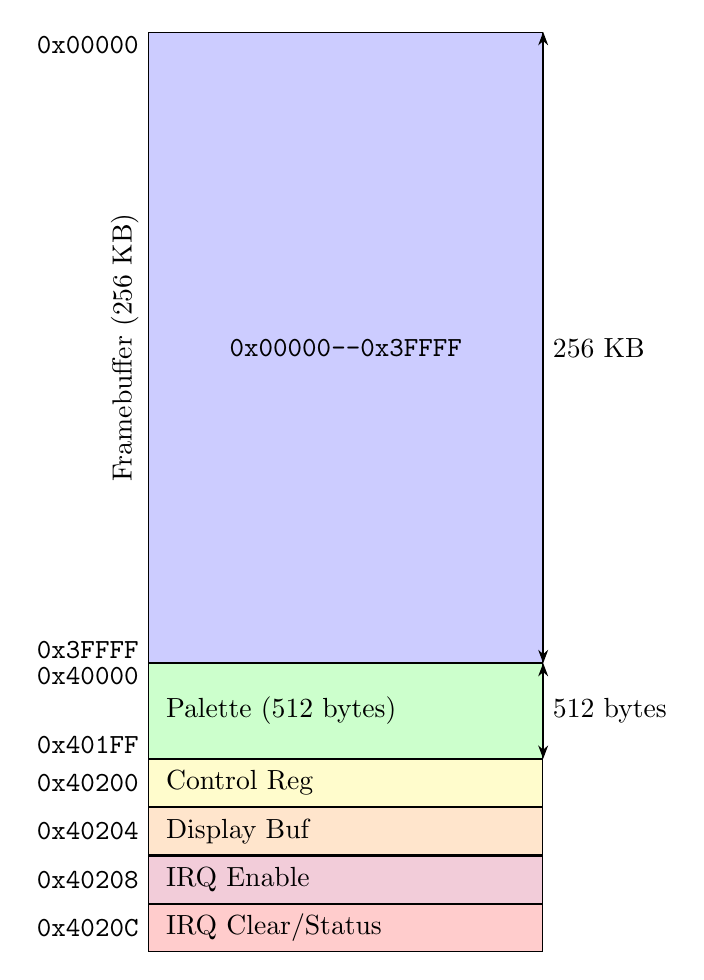
\begin{tikzpicture}[
    scale=1.0,
    memblock/.style={rectangle, draw, minimum width=5cm, anchor=north, font=\small}
]

% Memory blocks - properly sized and positioned
\node[memblock, minimum height=8cm, fill=blue!20] (fb) at (0, 0) {};
\node[above, rotate=90, anchor=south] at (fb.west) {Framebuffer (256 KB)};
\node at (fb.center) {\texttt{0x00000--0x3FFFF}};

% Palette - immediately after framebuffer, NO GAP
\node[memblock, minimum height=1.2cm, fill=green!20] (pal) at (fb.south) {};
\node[right=0.1cm] at (pal.west) {Palette (512 bytes)};

% Control registers - immediately after palette, NO GAP
\node[memblock, minimum height=0.6cm, fill=yellow!20] (ctrl) at (pal.south) {};
\node[right=0.1cm] at (ctrl.west) {Control Reg};

\node[memblock, minimum height=0.6cm, fill=orange!20] (disp) at (ctrl.south) {};
\node[right=0.1cm] at (disp.west) {Display Buf};

\node[memblock, minimum height=0.6cm, fill=purple!20] (irq) at (disp.south) {};
\node[right=0.1cm] at (irq.west) {IRQ Enable};

\node[memblock, minimum height=0.6cm, fill=red!20] (irqclr) at (irq.south) {};
\node[right=0.1cm] at (irqclr.west) {IRQ Clear/Status};

% Address labels on left
\node[left, yshift=-0.4\baselineskip] at (fb.north west) {\texttt{0x00000}};
\node[left, yshift=0.4\baselineskip] at (fb.south west) {\texttt{0x3FFFF}};
\node[left, yshift=-0.4\baselineskip] at (pal.north west) {\texttt{0x40000}};
\node[left, yshift=0.4\baselineskip] at (pal.south west) {\texttt{0x401FF}};
\node[left] at (ctrl.west) {\texttt{0x40200}};
\node[left] at (disp.west) {\texttt{0x40204}};
\node[left] at (irq.west) {\texttt{0x40208}};
\node[left] at (irqclr.west) {\texttt{0x4020C}};

% Size annotations
\draw[<->, >=Stealth] (fb.north east) -- (fb.south east) node[midway, right] {256 KB};
\draw[<->, >=Stealth] (pal.north east) -- (pal.south east) node[midway, right] {512 bytes};

\end{tikzpicture}
\caption{Memory Map Visualization}
\label{fig:memmap}
\end{figure}

\begin{longtable}{llp{6cm}}
\caption{Complete Memory Map} \label{tab:memmap} \\
\toprule
\textbf{Address Range} & \textbf{Size} & \textbf{Description} \\
\midrule
\endfirsthead

\multicolumn{3}{c}{\tablename\ \thetable\ -- continued from previous page} \\
\toprule
\textbf{Address Range} & \textbf{Size} & \textbf{Description} \\
\midrule
\endhead

\midrule
\multicolumn{3}{r}{Continued on next page} \\
\endfoot

\bottomrule
\endlastfoot

\texttt{0x00000--0x3FFFF} & 256 KB & Framebuffer Memory \\
\texttt{0x40000--0x401FF} & 512 bytes & Color Palette (256 entries) \\
\texttt{0x40200--0x40203} & 4 bytes & Control Register \\
\texttt{0x40204--0x40207} & 4 bytes & Display Buffer Select Register \\
\texttt{0x40208--0x4020B} & 4 bytes & IRQ Enable Register \\
\texttt{0x4020C--0x4020F} & 4 bytes & IRQ Clear/Status Register \\
\end{longtable}

\section{Framebuffer Memory (\texttt{0x00000--0x3FFFF})}

The framebuffer stores pixel data as 8-bit indexed color values. Each byte represents one pixel and is used as an index into the color palette.

\subsection{Memory Layout}

Pixels are stored in row-major order:

\begin{equation}
\text{Address} = y \times \text{width} + x
\end{equation}

Where:
\begin{itemize}
    \item $x$ is the horizontal pixel coordinate (0 to width-1)
    \item $y$ is the vertical pixel coordinate (0 to height-1)
    \item width is 320 (low-res mode) or 640 (high-res mode)
\end{itemize}

\subsection{320$\times$200 Mode (Double-Buffered)}

In 320$\times$200 mode, the framebuffer is divided into two buffers for double-buffering support as shown in Figure~\ref{fig:doublebuf_layout}:

\begin{figure}[tbp]
\centering
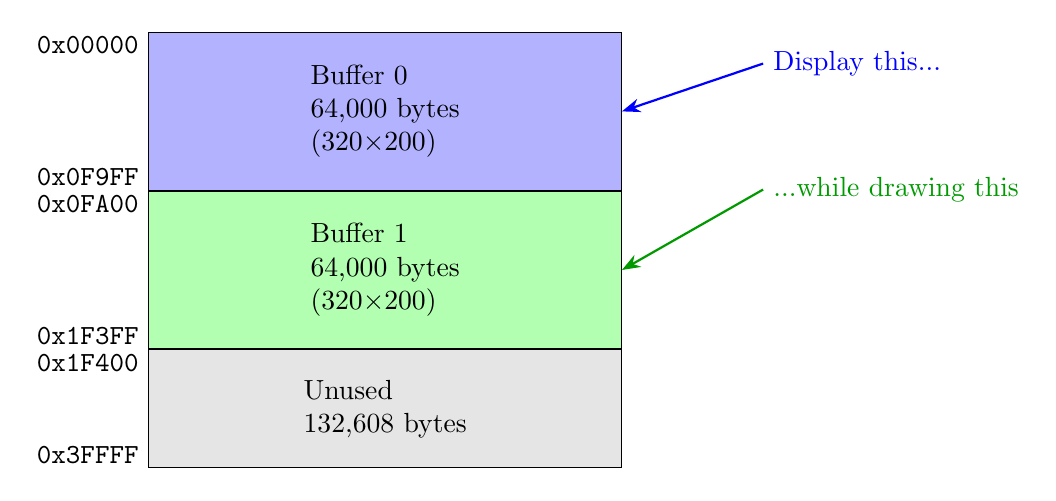
\begin{tikzpicture}[
    scale=0.8,
    memblock/.style={rectangle, draw, minimum width=6cm, anchor=north, font=\small}
]

% Buffer 0
\node[memblock, minimum height=2cm, fill=blue!30] (buf0) at (0, 0) {};
\node at (buf0.center) {\begin{varwidth}{\textwidth}Buffer 0\\64,000 bytes\\(320$\times$200)\end{varwidth}};
\node[left, yshift=-0.4\baselineskip] at (buf0.north west) {\texttt{0x00000}};
\node[left, yshift=0.4\baselineskip] at (buf0.south west) {\texttt{0x0F9FF}};
% Unused
%\node[memblock, minimum height=1cm, fill=gray!20] (unused1) at (buf0.south) {};
%\node at (unused1.center) {\begin{varwidth}{\textwidth}Unused\\1,536 bytes\end{varwidth}};
%\node[left, yshift=-0.4\baselineskip] at (unused1.north west) {\texttt{0x0FA00}};
%\node[left, yshift=1.4\baselineskip] at (unused1.south west) {\texttt{0x1FFFF}};
% Buffer 1
\node[memblock, minimum height=2cm, fill=green!30] (buf1) at (buf0.south) {};
\node at (buf1.center) {\begin{varwidth}{\textwidth}Buffer 1\\64,000 bytes\\(320$\times$200)\end{varwidth}};
\node[left, yshift=-0.4\baselineskip] at (buf1.north west) {\texttt{0x0FA00}};
\node[left, yshift=0.4\baselineskip] at (buf1.south west) {\texttt{0x1F3FF}};
% Unused
\node[memblock, minimum height=1.5cm, fill=gray!20] (unused) at (buf1.south) {};
\node at (unused.center) {\begin{varwidth}{\textwidth}Unused\\132,608 bytes\end{varwidth}};
\node[left, yshift=-0.4\baselineskip] at (unused.north west) {\texttt{0x1F400}};
\node[left, yshift=0.4\baselineskip] at (unused.south west) {\texttt{0x3FFFF}};
% Annotations
\draw[->, >=Stealth, thick, blue] (6, -0.5) -- (buf0.east) node[right, pos=0, blue] {Display this...};
\draw[->, >=Stealth, thick, green!60!black] (6, -2.5) -- (buf1.east) node[right, pos=0, green!60!black] {...while drawing this};

\end{tikzpicture}
\caption{320$\times$200 Double-Buffer Layout}
\label{fig:doublebuf_layout}
\end{figure}


\begin{table}[tbp]
\centering
\caption{320$\times$200 Framebuffer Layout}
\label{tab:fb_320_layout}
\begin{tabular}{lll}
\toprule
\textbf{Buffer} & \textbf{Address Range} & \textbf{Size} \\
\midrule
Buffer 0 & \texttt{0x00000--0x0F9FF} & 64,000 bytes \\
Buffer 1 & \texttt{0x0FA00--0x1F3FF} & 64,000 bytes \\
Unused   & \texttt{0x1F400--0x3FFFF} & 132,608 bytes \\
\bottomrule
\end{tabular}
\end{table}

\textbf{Address Calculation Example:}

To write a pixel at coordinates (x=100, y=50) to Buffer 1:

\begin{equation}
\begin{aligned}
\text{Address} &= \text{Buffer}_1\text{\_Base} + (y \times 320 + x) \\
               &= \texttt{0x0FA00} + (50 \times 320 + 100) \\
               &= \texttt{0x0FA00} + 16100 \\
               &= \texttt{0x13DE4}
\end{aligned}
\end{equation}

\subsection{640$\times$400 Mode (Single Buffer)}

In 640$\times$400 mode, a single framebuffer occupies the lower portion of memory:

\begin{table}[tbp]
\centering
\caption{640$\times$400 Framebuffer Layout}
\label{tab:fb_640_layout}
\begin{tabular}{lll}
\toprule
\textbf{Region} & \textbf{Address Range} & \textbf{Size} \\
\midrule
Framebuffer & \texttt{0x00000--0x3E7FF} & 256,000 bytes \\
Unused & \texttt{0x3E800--0x3FFFF} & 6,144 bytes \\
\bottomrule
\end{tabular}
\end{table}

\textbf{Address Calculation Example:}

To write a pixel at coordinates (x=320, y=200):

\begin{equation}
\begin{aligned}
\text{Address} &= y \times 640 + x \\
               &= 200 \times 640 + 320 \\
               &= 128320 \\
               &= \texttt{0x1F520}
\end{aligned}
\end{equation}

\subsection{Access Characteristics}

\begin{itemize}
    \item \textbf{Write Access:} Supports byte, halfword, and word writes (1-4 bytes written sequentially)
    \item \textbf{Read Access:} Supports byte, halfword, and word reads (1-4 bytes read sequentially)
    \item \textbf{Width:} 8-bit pixels (one byte per pixel)
    \item \textbf{Alignment:} Byte-addressable, no alignment restrictions
    \item \textbf{Write Latency:} 2 AXI cycles (single byte), 3-5 cycles (multi-byte sequential)
    \item \textbf{Read Latency:} 2 AXI cycles (single byte), 3-5 cycles (multi-byte sequential)
    \item \textbf{Byte Enables:} Supported for partial writes
\end{itemize}

\textbf{Multi-byte Read/Write:} The framebuffer supports efficient multi-byte reads and writes. When reading or writing words (4 bytes) or halfwords (2 bytes), the AXI slave sequentially accesses consecutive framebuffer addresses while holding the bus busy. This provides optimal performance for bulk operations.

\section{Color Palette (\texttt{0x40000--0x401FF})}

The color palette translates 8-bit pixel indices to 12-bit RGB colors.

\subsection{Palette Entry Format}

Each palette entry is 16 bits wide (16-bit halfword aligned in memory) as detailed in Table~\ref{tab:palette_bits}:

\begin{table}[tbp]
\centering
\caption{Palette Entry Bit Fields}
\label{tab:palette_bits}
\begin{tabular}{ccp{6cm}}
\toprule
\textbf{Bits} & \textbf{Field} & \textbf{Description} \\
\midrule
15--12 & Reserved & Must be written as 0 \\
11--8 & Red & Red channel intensity (0--15) \\
7--4 & Green & Green channel intensity (0--15) \\
3--0 & Blue & Blue channel intensity (0--15) \\
\bottomrule
\end{tabular}
\end{table}

\subsection{Palette Addressing}

Palette entries are accessed at word-aligned addresses:

\begin{equation}
\text{Palette Address} = \texttt{0x40000} + (\text{color\_index} \times 2)
\end{equation}

\textbf{Example:} To set color index 5 to bright red (RGB = F00):

\begin{lstlisting}[style=c]
uint16_t *palette = (uint16_t*)0x48040000;  // Base + palette offset
palette[5] = 0x0F00;  // Bright red
\end{lstlisting}

\subsection{Default Palette}

On reset, all palette entries are initialized to black (0x000). You must program the palette before meaningful colors appear.

\subsection{Standard VGA Colors}

A common starting palette uses the 16 standard VGA colors shown in Table~\ref{tab:standardpalette}.

\begin{table}[tbp]
\centering
\caption{Standard 16-Color VGA Palette}
\label{tab:standardpalette}
\begin{tabular}{clc}
\toprule
\textbf{Index} & \textbf{Color Name} & \textbf{RGB Value} \\
\midrule
0 & Black & \texttt{0x000} \\
1 & Blue & \texttt{0x00A} \\
2 & Green & \texttt{0x0A0} \\
3 & Cyan & \texttt{0x0AA} \\
4 & Red & \texttt{0xA00} \\
5 & Magenta & \texttt{0xA0A} \\
6 & Brown & \texttt{0xA50} \\
7 & Light Gray & \texttt{0xAAA} \\
8 & Dark Gray & \texttt{0x555} \\
9 & Bright Blue & \texttt{0x00F} \\
10 & Bright Green & \texttt{0x0F0} \\
11 & Bright Cyan & \texttt{0x0FF} \\
12 & Bright Red & \texttt{0xF00} \\
13 & Bright Magenta & \texttt{0xF0F} \\
14 & Yellow & \texttt{0xFF0} \\
15 & White & \texttt{0xFFF} \\
\bottomrule
\end{tabular}
\end{table}

\chapter{Register Descriptions}
\label{ch:registers}

\section{Control Register (\texttt{0x40200})}

The Control Register configures the basic operating mode of the VGA controller. Table~\ref{tab:ctrl_bits} shows the bit field definitions.

\subsection{Register Fields}

\begin{bytefield}[bitwidth=0.03\linewidth]{32}
\bitheader[endianness=big]{0-31} \\
\bitbox{31}{\tiny Reserved (RAZ/WI)} & \bitbox{1}{\tiny MODE}
\end{bytefield}

\begin{table}[tbp]
\centering
\caption{Control Register Bit Fields}
\label{tab:ctrl_bits}
\begin{tabular}{cllp{5cm}}
\toprule
\textbf{Bit} & \textbf{Name} & \textbf{Type} & \textbf{Description} \\
\midrule
0 & MODE & R/W & Resolution mode select \\
  &      &     & 0 = 640$\times$400 mode \\
  &      &     & 1 = 320$\times$200 mode \\
31--1 & -- & RAZ/WI & Reserved (Read-As-Zero, Write-Ignored) \\
\bottomrule
\end{tabular}
\end{table}

\subsection{Reset Value}

\texttt{0x00000000} (640$\times$400 mode)

\subsection{Usage Example}

\begin{lstlisting}[style=c,caption={Setting Display Mode}]
#define CTRL_REG  0x48040200

// Switch to 320x200 mode
*(volatile uint32_t*)CTRL_REG = 0x00000001;

// Switch to 640x400 mode
*(volatile uint32_t*)CTRL_REG = 0x00000000;

// Read current mode
uint32_t mode = *(volatile uint32_t*)CTRL_REG;
if (mode & 0x01) {
    printf("320x200 mode\n");
} else {
    printf("640x400 mode\n");
}
\end{lstlisting}

\subsection{Notes}

\begin{itemize}
    \item Mode changes take effect immediately but may cause visual glitches
    \item It's recommended to change modes during vertical blanking
    \item When switching from 320$\times$200 to 640$\times$400, the active buffer setting is ignored
    \item Framebuffer contents are not cleared when changing modes
\end{itemize}

\section{Display Buffer Register (\texttt{0x40204})}

The Display Buffer Register selects which framebuffer is displayed in 320$\times$200 mode. This enables double-buffering for flicker-free animation as shown in Table~\ref{tab:dispbuf_bits}.

\subsection{Register Fields}

\begin{bytefield}[bitwidth=0.03\linewidth]{32}
\bitheader[endianness=big]{0-31} \\
\bitbox{31}{\tiny Reserved (RAZ/WI)} & \bitbox{1}{\tiny BUF}
\end{bytefield}

\begin{table}[tbp]
\centering
\caption{Display Buffer Register Bit Fields}
\label{tab:dispbuf_bits}
\begin{tabular}{cllp{5cm}}
\toprule
\textbf{Bit} & \textbf{Name} & \textbf{Type} & \textbf{Description} \\
\midrule
0 & BUF & R/W & Display buffer select \\
  &     &     & 0 = Display Buffer 0 \\
  &     &     & 1 = Display Buffer 1 \\
  &     &     & (320$\times$200 mode only) \\
31--1 & -- & RAZ/WI & Reserved \\
\bottomrule
\end{tabular}
\end{table}

\subsection{Reset Value}

\texttt{0x00000000} (Buffer 0 displayed)

\subsection{Usage Example}

\begin{lstlisting}[style=c,caption={Double-Buffering Example}]
#define DISP_BUF_REG  0x48040204

uint8_t current_display_buffer = 0;
uint8_t current_draw_buffer = 1;

void swap_buffers(void) {
    // Swap the buffer being displayed
    current_display_buffer = current_draw_buffer;
    current_draw_buffer = 1 - current_draw_buffer;
    
    // Update hardware register (instant swap)
    *(volatile uint32_t*)DISP_BUF_REG = current_display_buffer;
}

// In your main animation loop:
while (1) {
    // Draw to the off-screen buffer
    draw_frame(current_draw_buffer);
    
    // Swap buffers (no tearing!)
    swap_buffers();
    
    // Optional: wait for vsync
    wait_for_vsync();
}
\end{lstlisting}

\subsection{Notes}

\begin{itemize}
    \item \textbf{Immediate switching:} Buffer switching is instantaneous - the change takes effect on the very next pixel being displayed
    \item \textbf{Warning:} Switching mid-frame will cause visible tearing (a horizontal line where the buffer change occurred)
    \item \textbf{Recommended practice:} Always swap buffers during vertical blanking using the VSYNC interrupt for tear-free animation
    \item This register has no effect in 640$\times$400 mode
    \item Reading this register returns the currently displayed buffer
\end{itemize}

\section{IRQ Enable Register (\texttt{0x40208})}

The IRQ Enable Register controls whether the VSYNC interrupt is forwarded to the processor. The interrupt fires at the beginning of the vertical blanking interval, making it ideal for synchronizing double-buffer swaps and other timing-critical operations.

\subsection{Register Fields}

\begin{bytefield}[bitwidth=0.03\linewidth]{32}
\bitheader[endianness=big]{0-31} \\
\bitbox{31}{\tiny Reserved (RAZ/WI)} & \bitbox{1}{\tiny VSIEN}
\end{bytefield}

\begin{table}[tbp]
\centering
\caption{IRQ Enable Register Bit Fields}
\label{tab:irqen_bits}
\begin{tabular}{cllp{6cm}}
\toprule
\textbf{Bit} & \textbf{Name} & \textbf{Type} & \textbf{Description} \\
\midrule
0 & VSIEN & R/W & Vertical Sync Interrupt Enable \\
  &       &     & 0 = Interrupt output disabled \\
  &       &     & 1 = Interrupt output enabled \\
31--1 & -- & RAZ/WI & Reserved \\
\bottomrule
\end{tabular}
\end{table}

\subsection{Reset Value}

\texttt{0x00000000} (Interrupt disabled)

\subsection{Notes}

\begin{itemize}
    \item VSIEN gates the \texttt{irq} output: \texttt{irq} = VSIEN AND VSIA
    \item Clearing VSIEN does \textit{not} clear the pending flag in the IRQ Clear/Status Register
    \item When VSIEN is re-enabled, any pending event that occurred while disabled will immediately assert \texttt{irq}
    \item Write 0 to this register to disable the interrupt at any time
\end{itemize}

\section{IRQ Clear/Status Register (\texttt{0x4020C})}

The IRQ Clear/Status Register reflects the current VSYNC interrupt pending state and provides the write-1-to-clear mechanism for acknowledging the interrupt. Reading this register allows software to poll for VSYNC without using the interrupt output. Table~\ref{tab:irqclr_bits} details the bit field definitions.

\subsection{Register Fields}

\begin{bytefield}[bitwidth=0.03\linewidth]{32}
\bitheader[endianness=big]{0-31} \\
\bitbox{31}{\tiny Reserved (RAZ/WI)} & \bitbox{1}{\tiny VSIA}
\end{bytefield}

\begin{table}[tbp]
\centering
\caption{IRQ Clear/Status Register Bit Fields}
\label{tab:irqclr_bits}
\begin{tabular}{cllp{6cm}}
\toprule
\textbf{Bit} & \textbf{Name} & \textbf{Type} & \textbf{Description} \\
\midrule
0 & VSIA & R/W1C & Vertical Sync Interrupt Active \\
  &      &       & 0 = No interrupt pending \\
  &      &       & 1 = Interrupt pending \\
  &      &       & Write 1 to clear; writing 0 has no effect \\
31--1 & -- & RAZ/WI & Reserved \\
\bottomrule
\end{tabular}
\end{table}

\subsection{Operation}

\textbf{Interrupt Generation:}
\begin{itemize}
    \item VSIA is automatically set on the rising edge of VSYNC (start of vertical blanking)
    \item The \texttt{irq} output = VSIEN (from IRQ Enable Register) AND VSIA
    \item The interrupt remains asserted until software clears VSIA
    \item VSIA is set regardless of whether VSIEN is enabled
\end{itemize}

\textbf{Clearing the Interrupt:}
\begin{itemize}
    \item Write \texttt{0x00000001} to this register to clear VSIA
    \item Writing 0 to bit 0 has no effect (write-1-to-clear semantics)
    \item The NVIC pending bit must also be cleared in the interrupt handler
\end{itemize}

\subsection{Reset Value}

\texttt{0x00000000} (No interrupt pending)

\subsection{Usage Example}

\begin{lstlisting}[style=c,caption={Interrupt-Driven Double-Buffering}]
#define VGA_BASE            0x48000000
#define VGA_IRQ_ENABLE_REG  (VGA_BASE + 0x40208)  // VSIEN at bit 0
#define VGA_IRQ_CLEAR_REG   (VGA_BASE + 0x4020C)  // VSIA  at bit 0 (R/W1C)
#define VGA_DISP_BUF_REG    (VGA_BASE + 0x40204)

// Enable VGA VSYNC interrupt
void vga_enable_irq(void) {
    *(volatile uint32_t*)VGA_IRQ_ENABLE_REG = 0x01;  // Set VSIEN
}

// VGA interrupt handler (called on VSYNC rising edge)
void vga_irq_handler(void) {
    // Check VSIA in the Clear/Status register
    if (*(volatile uint32_t*)VGA_IRQ_CLEAR_REG & 0x01) {
        // VSYNC occurred -- safe to swap buffers now
        static uint8_t display_buffer = 0;
        display_buffer ^= 1;
        *(volatile uint32_t*)VGA_DISP_BUF_REG = display_buffer;

        // Acknowledge: write 1 to bit 0 of IRQ Clear/Status register
        *(volatile uint32_t*)VGA_IRQ_CLEAR_REG = 0x01;
    }
}

// Main application
int main(void) {
    vga_enable_irq();
    register_interrupt_handler(VGA_IRQ_NUM, vga_irq_handler);
    enable_global_interrupts();

    while (1) {
        // Draw to off-screen buffer
        // Buffer swap happens automatically in the IRQ handler
        draw_next_frame();
    }
}
\end{lstlisting}

\subsection{Typical Use Case: Tear-Free Graphics}

The interrupt-driven approach ensures buffer swaps occur exclusively during vertical blanking:

\begin{enumerate}
    \item Write 1 to VSIEN in the IRQ Enable Register
    \item Draw graphics to the off-screen buffer
    \item On VSYNC interrupt:
    \begin{itemize}
        \item Swap the Display Buffer Register (no tearing --- the scan-out is in blanking)
        \item Optionally trigger audio or timing updates
        \item Write \texttt{0x01} to the IRQ Clear/Status Register to clear VSIA
    \end{itemize}
    \item Repeat
\end{enumerate}

\subsection{Notes}

\begin{itemize}
    \item The interrupt fires at approximately 70 Hz (once per frame)
    \item VSYNC occurs during the vertical blanking interval when no pixels are being drawn
    \item This is the optimal time to swap buffers for tear-free animation
    \item The interrupt handler should be kept short to avoid missing the blanking window
    \item Reading bit 0 of this register returns the current pending status
    \item The \texttt{irq} output connects to your processor's interrupt controller
\end{itemize}

\section{Status Registers (Future)}

The current version does not include status registers, but future versions may add:

\begin{itemize}
    \item V-SYNC status bit (for software synchronization)
    \item Frame counter
    \item Performance counters
\end{itemize}

\chapter{Programming Guide}
\label{ch:programming}

\section{Software Architecture}

This chapter provides complete programming information for the VGA controller, including initialization, drawing primitives, and advanced techniques.

\section{Initialization}

\subsection{Memory-Mapped Base Address}

First, define the base address where the VGA controller is mapped in your system:

\begin{lstlisting}[style=c]
// Adjust this address to match your system configuration
#define VGA_BASE            0x48000000

// Derived addresses
#define FB_BASE             (VGA_BASE + 0x00000)
#define FB_BUFFER_0         (FB_BASE  + 0x00000)  // 320x200 buffer 0
#define FB_BUFFER_1         (FB_BASE  + 0x0FA00)  // 320x200 buffer 1 (offset 64,000 bytes)
#define PALETTE_BASE        (VGA_BASE + 0x40000)
#define CTRL_REG            (VGA_BASE + 0x40200)
#define DISP_BUF_REG        (VGA_BASE + 0x40204)
#define VGA_IRQ_ENABLE_REG  (VGA_BASE + 0x40208)  // VSIEN at bit 0
#define VGA_IRQ_CLEAR_REG   (VGA_BASE + 0x4020C)  // VSIA  at bit 0 (R/W1C)
\end{lstlisting}

\subsection{Basic Initialization Sequence}

\begin{lstlisting}[style=c,caption={VGA Controller Initialization}]
void vga_init(void) {
    // 1. Set display mode
    *(volatile uint32_t*)CTRL_REG = 0x00000001;  // 320x200 mode
    
    // 2. Initialize palette with default colors
    init_palette();
    
    // 3. Clear both buffers
    clear_buffer(0);
    clear_buffer(1);
    
    // 4. Select buffer 0 for display
    *(volatile uint32_t*)DISP_BUF_REG = 0x00000000;
}

void clear_buffer(uint8_t buffer) {
    volatile uint8_t *fb;
    
    if (buffer == 0) {
        fb = (volatile uint8_t*)FB_BUFFER_0;
    } else {
        fb = (volatile uint8_t*)FB_BUFFER_1;
    }
    
    // Clear 64,000 bytes (320x200)
    for (int i = 0; i < 64000; i++) {
        fb[i] = 0;  // Black (assuming palette[0] is black)
    }
}
\end{lstlisting}

\subsection{Palette Initialization}

\begin{lstlisting}[style=c,caption={Standard VGA Palette Initialization}]
void init_palette(void) {
    volatile uint32_t *palette = (volatile uint32_t*)PALETTE_BASE;
    
    // Standard 16-color VGA palette
    palette[0]  = 0x000;  // Black
    palette[1]  = 0x00A;  // Blue
    palette[2]  = 0x0A0;  // Green
    palette[3]  = 0x0AA;  // Cyan
    palette[4]  = 0xA00;  // Red
    palette[5]  = 0xA0A;  // Magenta
    palette[6]  = 0xA50;  // Brown
    palette[7]  = 0xAAA;  // Light Gray
    palette[8]  = 0x555;  // Dark Gray
    palette[9]  = 0x00F;  // Bright Blue
    palette[10] = 0x0F0;  // Bright Green
    palette[11] = 0x0FF;  // Bright Cyan
    palette[12] = 0xF00;  // Bright Red
    palette[13] = 0xF0F;  // Bright Magenta
    palette[14] = 0xFF0;  // Yellow
    palette[15] = 0xFFF;  // White
    
    // Fill remaining entries with grayscale
    for (int i = 16; i < 256; i++) {
        uint8_t gray = i;  // 0-255 range
        uint8_t level = gray >> 4;  // Convert to 0-15
        palette[i] = (level << 8) | (level << 4) | level;
    }
}
\end{lstlisting}

\section{Drawing Primitives}

\subsection{Plot Pixel}

\begin{lstlisting}[style=c,caption={Pixel Plotting Function}]
void plot_pixel_320(uint16_t x, uint16_t y, 
                    uint8_t color, uint8_t buffer) {
    if (x >= 320 || y >= 200) return;  // Bounds check
    
    volatile uint8_t *fb;
    if (buffer == 0) {
        fb = (volatile uint8_t*)FB_BUFFER_0;
    } else {
        fb = (volatile uint8_t*)FB_BUFFER_1;
    }
    
    fb[y * 320 + x] = color;
}

void plot_pixel_640(uint16_t x, uint16_t y, uint8_t color) {
    if (x >= 640 || y >= 400) return;
    
    volatile uint8_t *fb = (volatile uint8_t*)FB_BASE;
    fb[y * 640 + x] = color;
}
\end{lstlisting}

\subsection{Read Pixel}

\begin{lstlisting}[style=c,caption={Reading Pixel Values}]
uint8_t get_pixel_320(uint16_t x, uint16_t y, uint8_t buffer) {
    if (x >= 320 || y >= 200) return 0;
    
    volatile uint8_t *fb;
    if (buffer == 0) {
        fb = (volatile uint8_t*)FB_BUFFER_0;
    } else {
        fb = (volatile uint8_t*)FB_BUFFER_1;
    }
    
    return fb[y * 320 + x];
}
\end{lstlisting}

\subsection{Draw Line (Bresenham's Algorithm)}

\begin{lstlisting}[style=c,caption={Line Drawing}]
void draw_line(int x0, int y0, int x1, int y1, 
               uint8_t color, uint8_t buffer) {
    int dx = abs(x1 - x0);
    int dy = abs(y1 - y0);
    int sx = (x0 < x1) ? 1 : -1;
    int sy = (y0 < y1) ? 1 : -1;
    int err = dx - dy;
    
    while (1) {
        plot_pixel_320(x0, y0, color, buffer);
        
        if (x0 == x1 && y0 == y1) break;
        
        int e2 = 2 * err;
        if (e2 > -dy) {
            err -= dy;
            x0 += sx;
        }
        if (e2 < dx) {
            err += dx;
            y0 += sy;
        }
    }
}
\end{lstlisting}

\subsection{Draw Rectangle}

\begin{lstlisting}[style=c,caption={Rectangle Drawing}]
void draw_rect(int x, int y, int w, int h, 
               uint8_t color, uint8_t buffer) {
    // Top and bottom edges
    for (int i = 0; i < w; i++) {
        plot_pixel_320(x + i, y, color, buffer);
        plot_pixel_320(x + i, y + h - 1, color, buffer);
    }
    
    // Left and right edges
    for (int i = 0; i < h; i++) {
        plot_pixel_320(x, y + i, color, buffer);
        plot_pixel_320(x + w - 1, y + i, color, buffer);
    }
}

void fill_rect(int x, int y, int w, int h, 
               uint8_t color, uint8_t buffer) {
    volatile uint8_t *fb;
    if (buffer == 0) {
        fb = (volatile uint8_t*)FB_BUFFER_0;
    } else {
        fb = (volatile uint8_t*)FB_BUFFER_1;
    }
    
    for (int row = y; row < y + h; row++) {
        if (row < 0 || row >= 200) continue;
        
        for (int col = x; col < x + w; col++) {
            if (col < 0 || col >= 320) continue;
            fb[row * 320 + col] = color;
        }
    }
}
\end{lstlisting}

\subsection{Draw Circle (Midpoint Algorithm)}

\begin{lstlisting}[style=c,caption={Circle Drawing}]
void plot_circle_points(int xc, int yc, int x, int y, 
                        uint8_t color, uint8_t buffer) {
    plot_pixel_320(xc + x, yc + y, color, buffer);
    plot_pixel_320(xc - x, yc + y, color, buffer);
    plot_pixel_320(xc + x, yc - y, color, buffer);
    plot_pixel_320(xc - x, yc - y, color, buffer);
    plot_pixel_320(xc + y, yc + x, color, buffer);
    plot_pixel_320(xc - y, yc + x, color, buffer);
    plot_pixel_320(xc + y, yc - x, color, buffer);
    plot_pixel_320(xc - y, yc - x, color, buffer);
}

void draw_circle(int xc, int yc, int radius, 
                 uint8_t color, uint8_t buffer) {
    int x = 0;
    int y = radius;
    int d = 1 - radius;
    
    plot_circle_points(xc, yc, x, y, color, buffer);
    
    while (x < y) {
        x++;
        if (d < 0) {
            d += 2 * x + 1;
        } else {
            y--;
            d += 2 * (x - y) + 1;
        }
        plot_circle_points(xc, yc, x, y, color, buffer);
    }
}
\end{lstlisting}

\section{Advanced Techniques}

\subsection{Optimized Block Fill}

For better performance when filling large areas:

\begin{lstlisting}[style=c,caption={Optimized Block Fill Using memset}]
#include <string.h>

void fast_fill_rect(int x, int y, int w, int h, 
                    uint8_t color, uint8_t buffer) {
    volatile uint8_t *fb;
    if (buffer == 0) {
        fb = (volatile uint8_t*)FB_BUFFER_0;
    } else {
        fb = (volatile uint8_t*)FB_BUFFER_1;
    }
    
    for (int row = y; row < y + h; row++) {
        if (row < 0 || row >= 200) continue;
        
        int start_x = (x < 0) ? 0 : x;
        int end_x = (x + w > 320) ? 320 : x + w;
        int width = end_x - start_x;
        
        if (width > 0) {
            memset((void*)&fb[row * 320 + start_x], color, width);
        }
    }
}
\end{lstlisting}

\subsection{Sprite Drawing}

\begin{lstlisting}[style=c,caption={Sprite Rendering with Transparency}]
typedef struct {
    int width;
    int height;
    const uint8_t *data;
} Sprite;

void draw_sprite(int x, int y, const Sprite *sprite, 
                 uint8_t buffer) {
    volatile uint8_t *fb;
    if (buffer == 0) {
        fb = (volatile uint8_t*)FB_BUFFER_0;
    } else {
        fb = (volatile uint8_t*)FB_BUFFER_1;
    }
    
    for (int row = 0; row < sprite->height; row++) {
        int screen_y = y + row;
        if (screen_y < 0 || screen_y >= 200) continue;
        
        for (int col = 0; col < sprite->width; col++) {
            int screen_x = x + col;
            if (screen_x < 0 || screen_x >= 320) continue;
            
            uint8_t pixel = sprite->data[row * sprite->width + col];
            
            // Color 0 is transparent
            if (pixel != 0) {
                fb[screen_y * 320 + screen_x] = pixel;
            }
        }
    }
}

// Example sprite data (8x8 smiley face)
const uint8_t smiley_data[64] = {
    0,0,15,15,15,15,0,0,
    0,15,14,14,14,14,15,0,
    15,14,1,14,14,1,14,15,
    15,14,14,14,14,14,14,15,
    15,14,1,14,14,1,14,15,
    15,14,14,1,1,14,14,15,
    0,15,14,14,14,14,15,0,
    0,0,15,15,15,15,0,0
};

const Sprite smiley = {
    .width = 8,
    .height = 8,
    .data = smiley_data
};
\end{lstlisting}

\subsection{Scrolling}

\begin{lstlisting}[style=c,caption={Vertical Scrolling}]
void scroll_up(int lines, uint8_t buffer) {
    volatile uint8_t *fb;
    if (buffer == 0) {
        fb = (volatile uint8_t*)FB_BUFFER_0;
    } else {
        fb = (volatile uint8_t*)FB_BUFFER_1;
    }
    
    // Move pixels up
    memmove((void*)fb, 
            (const void*)&fb[lines * 320], 
            (200 - lines) * 320);
    
    // Clear bottom lines
    memset((void*)&fb[(200 - lines) * 320], 0, lines * 320);
}
\end{lstlisting}

\section{Double-Buffering Example}

\begin{lstlisting}[style=c,caption={Complete Double-Buffering Application}]
#include <stdint.h>
#include <stdbool.h>

typedef struct {
    uint8_t display_buffer;
    uint8_t draw_buffer;
    bool vsync_enabled;
} VGA_State;

VGA_State vga_state = {0, 1, false};

void vga_swap_buffers(void) {
    // Swap display and draw buffers
    uint8_t temp = vga_state.display_buffer;
    vga_state.display_buffer = vga_state.draw_buffer;
    vga_state.draw_buffer = temp;
    
    // Update hardware register
    *(volatile uint32_t*)DISP_BUF_REG = vga_state.display_buffer;
}

uint8_t vga_get_draw_buffer(void) {
    return vga_state.draw_buffer;
}

// Example: Bouncing ball animation
typedef struct {
    float x, y;
    float vx, vy;
    uint8_t color;
    int radius;
} Ball;

void animate_ball(Ball *ball) {
    const int WIDTH = 320;
    const int HEIGHT = 200;
    
    while (1) {
        uint8_t buffer = vga_get_draw_buffer();
        
        // Clear screen
        fast_fill_rect(0, 0, WIDTH, HEIGHT, 0, buffer);
        
        // Update ball position
        ball->x += ball->vx;
        ball->y += ball->vy;
        
        // Bounce off walls
        if (ball->x - ball->radius < 0 || 
            ball->x + ball->radius >= WIDTH) {
            ball->vx = -ball->vx;
        }
        if (ball->y - ball->radius < 0 || 
            ball->y + ball->radius >= HEIGHT) {
            ball->vy = -ball->vy;
        }
        
        // Draw ball
        draw_circle((int)ball->x, (int)ball->y, 
                   ball->radius, ball->color, buffer);
        
        // Swap buffers (no tearing!)
        vga_swap_buffers();
        
        // Optional: delay for frame rate control
        delay_ms(16);  // ~60 FPS
    }
}

int main(void) {
    // Initialize VGA
    vga_init();
    
    // Create a ball
    Ball ball = {
        .x = 160,
        .y = 100,
        .vx = 2.5,
        .vy = 1.8,
        .color = 12,  // Bright red
        .radius = 8
    };
    
    // Run animation
    animate_ball(&ball);
    
    return 0;
}
\end{lstlisting}

\chapter{Display Modes}

\section{320$\times$200 Mode}

\subsection{Overview}

320$\times$200 mode provides a classic low-resolution mode suitable for retro gaming and applications where large pixels are desirable.

\subsection{Technical Details}

\begin{itemize}
    \item \textbf{Resolution:} 320$\times$200 pixels
    \item \textbf{Display:} Each pixel is doubled to 2$\times$2 screen pixels (640$\times$400 output)
    \item \textbf{Framebuffer Size:} 64,000 bytes per buffer
    \item \textbf{Double-Buffering:} Supported (two 64 KB buffers)
    \item \textbf{Refresh Rate:} 70 Hz
    \item \textbf{Colors:} 256 simultaneous from 4096-color palette
\end{itemize}

\subsection{Memory Usage}

\begin{table}[tbp]
\centering
\caption{320$\times$200 Mode Memory Allocation}
\label{tab:mem_320}
\begin{tabular}{lrr}
\toprule
\textbf{Resource} & \textbf{Size} & \textbf{Usage} \\
\midrule
Buffer 0 & 64,000 bytes & 25\% of 256 KB \\
Buffer 1 & 64,000 bytes & 25\% of 256 KB \\
Total Used & 128,000 bytes & 50\% of 256 KB \\
Available & 128,000 bytes & 50\% of 256 KB \\
\bottomrule
\end{tabular}
\end{table}

\subsection{Performance Characteristics}

\begin{itemize}
    \item \textbf{Pixel Update Rate:} Limited by AXI bus speed (typically 100 MHz)
    \item \textbf{Full Screen Update:} Can update entire framebuffer in \textless 1 ms
    \item \textbf{Buffer Swap:} Instantaneous (single register write)
    \item \textbf{Memory Bandwidth:} 4.48 MB/s for display reads
\end{itemize}

\subsection{Best Use Cases}

\begin{itemize}
    \item Retro-style games
    \item Pixel art applications
    \item Fast-paced animations requiring double-buffering
    \item Applications where memory is constrained
    \item Classic computer emulation
\end{itemize}

\section{640$\times$400 Mode}

\subsection{Overview}

640$\times$400 mode provides higher resolution for applications requiring more detail.

\subsection{Technical Details}

\begin{itemize}
    \item \textbf{Resolution:} 640$\times$400 pixels
    \item \textbf{Display:} 1:1 pixel mapping (no doubling)
    \item \textbf{Framebuffer Size:} 256,000 bytes
    \item \textbf{Double-Buffering:} Not supported (insufficient memory)
    \item \textbf{Refresh Rate:} 70 Hz
    \item \textbf{Colors:} 256 simultaneous from 4096-color palette
\end{itemize}

\subsection{Memory Usage}

\begin{table}[tbp]
\centering
\caption{640$\times$400 Mode Memory Allocation}
\label{tab:mem_640}
\begin{tabular}{lrr}
\toprule
\textbf{Resource} & \textbf{Size} & \textbf{Usage} \\
\midrule
Framebuffer & 256,000 bytes & 100\% of 256 KB \\
Available & 0 bytes & 0\% of 256 KB \\
\bottomrule
\end{tabular}
\end{table}

\subsection{Performance Characteristics}

\begin{itemize}
    \item \textbf{Full Screen Update:} ~2.5 ms at 100 MHz AXI clock
    \item \textbf{Memory Bandwidth:} 17.92 MB/s for display reads
    \item \textbf{Pixel Density:} 4$\times$ more pixels than 320$\times$200 mode
\end{itemize}

\subsection{Best Use Cases}

\begin{itemize}
    \item Text-based interfaces requiring higher resolution
    \item Detailed graphics applications
    \item CAD/drawing applications
    \item Data visualization
    \item Applications where double-buffering is not needed
\end{itemize}

\subsection{Handling Tearing Without Double-Buffering}

Since 640$\times$400 mode doesn't support double-buffering, you can minimize tearing by:

\begin{enumerate}
    \item Drawing only during vertical blanking (if you can draw fast enough)
    \item Using partial screen updates (only redraw changed regions)
    \item Implementing triple-buffering in external SDRAM
    \item Accepting some tearing for non-critical applications
\end{enumerate}

\section{Mode Comparison}

Table~\ref{tab:mode_compare} provides a detailed comparison of the two available display modes:

\begin{table}[tbp]
\centering
\caption{Display Mode Comparison}
\label{tab:mode_compare}
\begin{tabular}{lcc}
\toprule
\textbf{Feature} & \textbf{320$\times$200} & \textbf{640$\times$400} \\
\midrule
Pixels & 64,000 & 256,000 \\
Memory per Buffer & 64 KB & 256 KB \\
Double-Buffering & Yes & No \\
Pixel Size & 2$\times$2 (large) & 1$\times$1 (small) \\
Update Speed & Fast & Moderate \\
Memory Available & 50\% free & 0\% free \\
Best For & Games & Applications \\
\bottomrule
\end{tabular}
\end{table}

\chapter{Color Palette}

\section{Palette Architecture}

The VGA controller uses an indexed color system with a programmable palette.

\subsection{How It Works}

The indexed color pipeline is illustrated in Figure~\ref{fig:color_pipeline}:

\begin{enumerate}
    \item Each pixel in the framebuffer is 8 bits (0--255)
    \item This value is used as an index into the palette
    \item The palette entry contains a 12-bit RGB color
    \item The RGB color is output to the VGA DAC
\end{enumerate}

\begin{figure}[tbp]
\centering
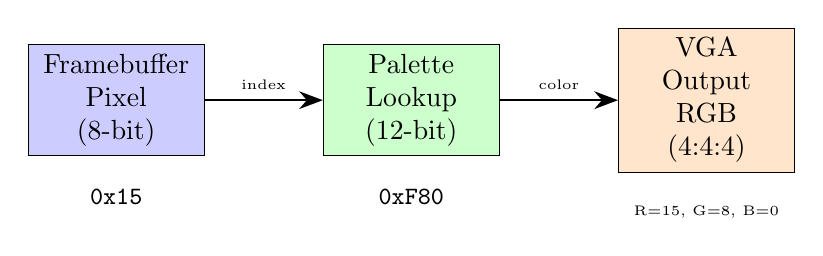
\begin{tikzpicture}[
    node distance=2cm,
    stage/.style={rectangle, draw, fill=blue!20, text width=2cm, text centered, minimum height=1cm},
    arrow/.style={-{Stealth[length=3mm]}, thick}
]

\node[stage] (fb) {Framebuffer\\Pixel\\(8-bit)};
\node[stage, right=1.5cm of fb, fill=green!20] (pal) {Palette\\Lookup\\(12-bit)};
\node[stage, right=1.5cm of pal, fill=orange!20] (rgb) {VGA Output\\RGB\\(4:4:4)};

\draw[arrow] (fb) -- node[above] {\tiny index} (pal);
\draw[arrow] (pal) -- node[above] {\tiny color} (rgb);

% Example values
\node[below=0.3cm of fb, font=\small] {\texttt{0x15}};
\node[below=0.3cm of pal, font=\small] {\texttt{0xF80}};
\node[below=0.3cm of rgb, font=\small\tiny] {R=15, G=8, B=0};

\end{tikzpicture}
\caption{Indexed Color Pipeline}
\label{fig:color_pipeline}
\end{figure}

\subsection{Advantages of Indexed Color}

\begin{itemize}
    \item \textbf{Memory Efficiency:} 1 byte per pixel vs 3 bytes for direct RGB
    \item \textbf{Fast Color Changes:} Change palette to recolor entire screen
    \item \textbf{Palette Animation:} Create effects by cycling palette entries
    \item \textbf{Color Standardization:} Use consistent colors across application
\end{itemize}

\section{Palette Programming}

\subsection{Setting Individual Colors}

\begin{lstlisting}[style=c,caption={Setting Palette Entries}]
void set_palette_entry(uint8_t index, 
                       uint8_t red, uint8_t green, uint8_t blue) {
    volatile uint32_t *palette = (volatile uint32_t*)PALETTE_BASE;
    
    // Combine RGB into 12-bit value (4 bits each)
    uint16_t rgb = ((red & 0x0F) << 8) | 
                   ((green & 0x0F) << 4) | 
                   (blue & 0x0F);
    
    palette[index] = rgb;
}

// Example: Set color 10 to orange
set_palette_entry(10, 15, 8, 0);  // RGB = F80
\end{lstlisting}

\subsection{Loading Complete Palettes}

\begin{lstlisting}[style=c,caption={Loading a Full Palette}]
typedef struct {
    uint8_t r, g, b;
} RGB;

void load_palette(const RGB *colors, int num_colors) {
    volatile uint32_t *palette = (volatile uint32_t*)PALETTE_BASE;
    
    for (int i = 0; i < num_colors && i < 256; i++) {
        uint16_t rgb = ((colors[i].r & 0x0F) << 8) | 
                       ((colors[i].g & 0x0F) << 4) | 
                       (colors[i].b & 0x0F);
        palette[i] = rgb;
    }
}

// Example: Earth tone palette
const RGB earth_palette[] = {
    {0, 0, 0},      // 0: Black
    {5, 3, 1},      // 1: Dark brown
    {8, 5, 2},      // 2: Brown
    {11, 8, 4},     // 3: Light brown
    {2, 6, 2},      // 4: Dark green
    {4, 10, 4},     // 5: Green
    {8, 13, 8},     // 6: Light green
    {10, 10, 15},   // 7: Sky blue
    {15, 15, 15},   // 8: White
};

load_palette(earth_palette, 9);
\end{lstlisting}

\section{Palette Techniques}

\subsection{Palette Fading}

\begin{lstlisting}[style=c,caption={Fade to Black Effect}]
void fade_to_black(int steps, int delay_ms) {
    RGB original_palette[256];
    volatile uint32_t *palette = (volatile uint32_t*)PALETTE_BASE;
    
    // Save original palette
    for (int i = 0; i < 256; i++) {
        uint16_t rgb = palette[i];
        original_palette[i].r = (rgb >> 8) & 0x0F;
        original_palette[i].g = (rgb >> 4) & 0x0F;
        original_palette[i].b = rgb & 0x0F;
    }
    
    // Fade out
    for (int step = steps; step >= 0; step--) {
        for (int i = 0; i < 256; i++) {
            uint8_t r = (original_palette[i].r * step) / steps;
            uint8_t g = (original_palette[i].g * step) / steps;
            uint8_t b = (original_palette[i].b * step) / steps;
            
            set_palette_entry(i, r, g, b);
        }
        delay_ms(delay_ms);
    }
}

// Restore original colors
void fade_from_black(const RGB *original, int steps, int delay_ms) {
    for (int step = 0; step <= steps; step++) {
        for (int i = 0; i < 256; i++) {
            uint8_t r = (original[i].r * step) / steps;
            uint8_t g = (original[i].g * step) / steps;
            uint8_t b = (original[i].b * step) / steps;
            
            set_palette_entry(i, r, g, b);
        }
        delay_ms(delay_ms);
    }
}
\end{lstlisting}

\subsection{Palette Rotation (Color Cycling)}

\begin{lstlisting}[style=c,caption={Water Effect Using Palette Rotation}]
void rotate_palette_range(uint8_t start, uint8_t end, int direction) {
    volatile uint32_t *palette = (volatile uint32_t*)PALETTE_BASE;
    
    if (direction > 0) {
        // Rotate forward
        uint16_t temp = palette[end];
        for (int i = end; i > start; i--) {
            palette[i] = palette[i-1];
        }
        palette[start] = temp;
    } else {
        // Rotate backward
        uint16_t temp = palette[start];
        for (int i = start; i < end; i++) {
            palette[i] = palette[i+1];
        }
        palette[end] = temp;
    }
}

// Example: Animated water using palette cycling
void animate_water(void) {
    // Set up blue gradient in palette entries 16-31
    for (int i = 0; i < 16; i++) {
        uint8_t blue_level = i;
        set_palette_entry(16 + i, 0, i/2, blue_level);
    }
    
    // Draw water area using colors 16-31
    fill_rect(0, 150, 320, 50, 20, get_draw_buffer());
    
    // Animate by rotating palette
    while (1) {
        rotate_palette_range(16, 31, 1);
        delay_ms(50);  // Animation speed
    }
}
\end{lstlisting}

\subsection{Grayscale Conversion}

\begin{lstlisting}[style=c,caption={Convert Palette to Grayscale}]
void palette_to_grayscale(void) {
    volatile uint32_t *palette = (volatile uint32_t*)PALETTE_BASE;
    
    for (int i = 0; i < 256; i++) {
        uint16_t rgb = palette[i];
        uint8_t r = (rgb >> 8) & 0x0F;
        uint8_t g = (rgb >> 4) & 0x0F;
        uint8_t b = rgb & 0x0F;
        
        // Convert to grayscale using luminance formula
        // Gray = 0.299*R + 0.587*G + 0.114*B
        uint8_t gray = (3*r + 6*g + 1*b) / 10;
        
        palette[i] = (gray << 8) | (gray << 4) | gray;
    }
}
\end{lstlisting}

\section{Common Palette Schemes}

\subsection{Web-Safe Colors (216 colors)}

\begin{lstlisting}[style=c,caption={Generate Web-Safe Palette}]
void generate_websafe_palette(void) {
    int index = 0;
    
    // 6x6x6 color cube
    for (int r = 0; r < 6; r++) {
        for (int g = 0; g < 6; g++) {
            for (int b = 0; b < 6; b++) {
                // Map 0-5 to 0-15 (4-bit)
                uint8_t red = (r * 15) / 5;
                uint8_t green = (g * 15) / 5;
                uint8_t blue = (b * 15) / 5;
                
                set_palette_entry(index++, red, green, blue);
                
                if (index >= 256) return;
            }
        }
    }
}
\end{lstlisting}

\chapter{Double-Buffering}

\section{Concept}

Double-buffering eliminates screen tearing by maintaining two framebuffers:

\begin{enumerate}
    \item \textbf{Display Buffer:} Currently visible on screen
    \item \textbf{Draw Buffer:} Being updated by the CPU
\end{enumerate}

When drawing is complete, the buffers are swapped instantly, making the newly drawn frame visible without tearing or flicker, as shown in Figure~\ref{fig:doublebuf_concept}.

\subsection{Visual Explanation}

\begin{figure}[tbp]
\centering
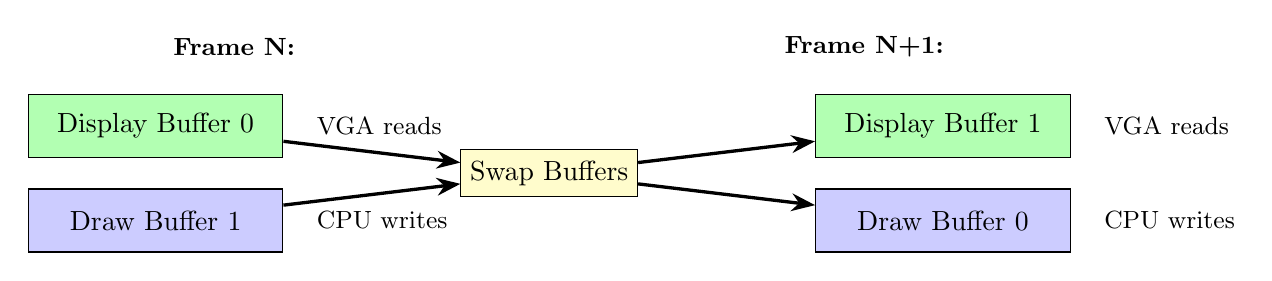
\begin{tikzpicture}[
    buffer/.style={rectangle, draw, fill=blue!20, text width=3cm, text centered, minimum height=0.8cm},
    arrow/.style={-{Stealth[length=2mm]}, thick},
    label/.style={font=\small}
]

% Frame N
\node[label] at (-4, 2.5) {\textbf{Frame N:}};
\node[buffer, fill=green!30] (disp0) at (-5, 1.5) {Display Buffer 0};
\node[buffer, fill=blue!20] (draw1) at (-5, 0.3) {Draw Buffer 1};

\node[label, right=0.3cm of disp0, anchor=west] {VGA reads};
\node[label, right=0.3cm of draw1, anchor=west] {CPU writes};

% Swap indicator
\node[draw, rectangle, fill=yellow!20, minimum width=2cm, minimum height=0.6cm] (swap) at (0, 0.9) {Swap Buffers};

% Frame N+1
\node[label] at (4, 2.5) {\textbf{Frame N+1:}};
\node[buffer, fill=green!30] (disp1) at (5, 1.5) {Display Buffer 1};
\node[buffer, fill=blue!20] (draw0) at (5, 0.3) {Draw Buffer 0};

\node[label, right=0.3cm of disp1, anchor=west] {VGA reads};
\node[label, right=0.3cm of draw0, anchor=west] {CPU writes};

\draw[-{Stealth[length=3mm]}, very thick] (disp0) -- (swap);
\draw[-{Stealth[length=3mm]}, very thick] (draw1) -- (swap);
\draw[-{Stealth[length=3mm]}, very thick] (swap) -- (disp1);
\draw[-{Stealth[length=3mm]}, very thick] (swap) -- (draw0);


\end{tikzpicture}
\caption{Double-Buffering Concept}
\label{fig:doublebuf_concept}
\end{figure}

\section{Implementation}

\subsection{Basic Double-Buffer Manager}

\begin{lstlisting}[style=c,caption={Double-Buffer Management}]
typedef struct {
    uint8_t front_buffer;  // Currently displayed
    uint8_t back_buffer;   // Currently being drawn
} DoubleBuffer;

DoubleBuffer db = {0, 1};

void db_swap(void) {
    // Swap the buffers
    uint8_t temp = db.front_buffer;
    db.front_buffer = db.back_buffer;
    db.back_buffer = temp;
    
    // Update hardware to display new front buffer
    *(volatile uint32_t*)DISP_BUF_REG = db.front_buffer;
}

uint8_t db_get_back_buffer(void) {
    return db.back_buffer;
}

uint8_t db_get_front_buffer(void) {
    return db.front_buffer;
}
\end{lstlisting}

\subsection{With V-Sync Synchronization}

\textbf{Important:} The Display Buffer Register changes take effect \textit{immediately} on the next pixel. Switching buffers mid-frame will cause visible screen tearing. To achieve tear-free animation, you \textit{must} swap buffers during the vertical blanking interval using the VSYNC interrupt:

\begin{lstlisting}[style=c,caption={V-Sync Synchronized Buffer Swap Using Interrupt}]
#define VGA_BASE            0x48000000
#define VGA_IRQ_ENABLE_REG  (VGA_BASE + 0x40208)  // VSIEN at bit 0
#define VGA_IRQ_CLEAR_REG   (VGA_BASE + 0x4020C)  // VSIA  at bit 0 (R/W1C)
#define DISP_BUF_REG        (VGA_BASE + 0x40204)

volatile uint8_t next_buffer = 0;
volatile uint8_t swap_pending = 0;

// Enable VSYNC interrupt
void init_vsync(void) {
    *(volatile uint32_t*)VGA_IRQ_ENABLE_REG = 0x01;  // Set VSIEN
}

// VSYNC interrupt handler - swaps happen here (during vertical blanking)
void vga_irq_handler(void) {
    // Check VSIA in the Clear/Status register
    if (*(volatile uint32_t*)VGA_IRQ_CLEAR_REG & 0x01) {
        // We're in vertical blanking - safe to swap now!
        if (swap_pending) {
            *(volatile uint32_t*)DISP_BUF_REG = next_buffer;
            swap_pending = 0;
        }

        // Acknowledge interrupt (W1C: write 1 to bit 0)
        *(volatile uint32_t*)VGA_IRQ_CLEAR_REG = 0x01;
    }
}

// Request a buffer swap (will happen on next VSYNC)
void db_swap_request(void) {
    next_buffer = 1 - next_buffer;  // Toggle buffer
    swap_pending = 1;               // Mark swap as pending
    // Actual swap happens in interrupt handler during vertical blanking
}

// Main animation loop
void animation_loop(void) {
    init_vsync();
    
    while (1) {
        // Draw to off-screen buffer
        draw_frame(1 - next_buffer);
        
        // Request buffer swap (happens on next VSYNC automatically)
        db_swap_request();
        
        // Continue - swap will happen in interrupt handler
    }
}

\end{lstlisting}

\textbf{Why This Works:}
\begin{itemize}
    \item The VSYNC interrupt fires during vertical blanking (when no pixels are being drawn)
    \item Swapping buffers during this time ensures the entire frame uses one consistent buffer
    \item No tearing occurs because the display never switches buffers mid-frame
    \item The interrupt-driven approach is more efficient than polling
\end{itemize}

\textbf{What Happens Without VSYNC Synchronization:}
\begin{itemize}
    \item If you write to the Display Buffer Register at any time, the change is \textit{immediate}
    \item The very next pixel displayed will come from the new buffer
    \item This creates a visible horizontal "tear line" where the buffer changed mid-frame
    \item Always use the interrupt handler approach shown above for tear-free graphics
\end{itemize}

\subsection{Game Loop with Double-Buffering}

\begin{lstlisting}[style=c,caption={Typical Game Loop}]
typedef struct {
    float x, y;
    float dx, dy;
} GameObject;

void game_loop(void) {
    GameObject player = {160, 100, 0, 0};
    GameObject enemies[10];
    
    // Initialize
    vga_init();
    init_game_objects(enemies, 10);
    
    while (!game_over) {
        uint8_t buffer = db_get_back_buffer();
        
        // 1. Process input
        process_input(&player);
        
        // 2. Update game state
        update_player(&player);
        update_enemies(enemies, 10);
        check_collisions(&player, enemies, 10);
        
        // 3. Render to back buffer
        clear_screen(buffer);
        draw_player(&player, buffer);
        draw_enemies(enemies, 10, buffer);
        draw_ui(buffer);
        
        // 4. Swap buffers (makes new frame visible)
        db_swap_vsync();
    }
}
\end{lstlisting}

\section{Advanced Double-Buffering Techniques}

\subsection{Partial Updates}

For static backgrounds, you can avoid redrawing the entire screen:

\begin{lstlisting}[style=c,caption={Partial Screen Updates}]
typedef struct {
    int x, y, w, h;
} DirtyRect;

#define MAX_DIRTY_RECTS 32

typedef struct {
    DirtyRect rects[MAX_DIRTY_RECTS];
    int count;
} DirtyRegions;

DirtyRegions dirty = {0};

void mark_dirty(int x, int y, int w, int h) {
    if (dirty.count < MAX_DIRTY_RECTS) {
        dirty.rects[dirty.count].x = x;
        dirty.rects[dirty.count].y = y;
        dirty.rects[dirty.count].w = w;
        dirty.rects[dirty.count].h = h;
        dirty.count++;
    }
}

void update_dirty_regions(uint8_t src_buffer, uint8_t dst_buffer) {
    volatile uint8_t *src_fb = (src_buffer == 0) ? 
        (volatile uint8_t*)FB_BUFFER_0 : 
        (volatile uint8_t*)FB_BUFFER_1;
    volatile uint8_t *dst_fb = (dst_buffer == 0) ? 
        (volatile uint8_t*)FB_BUFFER_0 : 
        (volatile uint8_t*)FB_BUFFER_1;
    
    for (int i = 0; i < dirty.count; i++) {
        DirtyRect *r = &dirty.rects[i];
        
        for (int y = r->y; y < r->y + r->h; y++) {
            memcpy((void*)&dst_fb[y * 320 + r->x],
                   (const void*)&src_fb[y * 320 + r->x],
                   r->w);
        }
    }
    
    dirty.count = 0;
}
\end{lstlisting}

\subsection{Triple Buffering (Using External RAM)}

If you have external SDRAM, you can implement triple buffering:

\begin{lstlisting}[style=c,caption={Triple Buffering Concept}]
// Three buffers:
// - Buffer 0: Internal BRAM (currently displayed)
// - Buffer 1: Internal BRAM (ready to display)
// - Buffer 2: External SDRAM (being drawn)

typedef struct {
    uint8_t display_buffer;   // Currently on screen
    uint8_t ready_buffer;     // Ready to display
    uint8_t draw_buffer;      // Being drawn (in SDRAM)
} TripleBuffer;

TripleBuffer tb = {0, 1, 2};

void tb_swap(void) {
    // Move ready buffer to display
    tb.display_buffer = tb.ready_buffer;
    *(volatile uint32_t*)DISP_BUF_REG = tb.display_buffer;
    
    // Copy finished frame from SDRAM to ready buffer
    memcpy((void*)get_buffer_address(tb.ready_buffer),
           (void*)SDRAM_BUFFER_2,
           64000);
    
    // Rotate buffers
    uint8_t temp = tb.draw_buffer;
    tb.draw_buffer = tb.ready_buffer;
    tb.ready_buffer = temp;
}
\end{lstlisting}

\chapter{Hardware Integration}

\section{Connecting to a MicroBlaze Processor}

\subsection{Block Design Creation}

\begin{enumerate}
    \item In Vivado, create a new Block Design
    \item Add MicroBlaze processor IP
    \item Run Block Automation (accept defaults)
    \item Add VGA Controller:
    \begin{itemize}
        \item Right-click in canvas, then Add Module
        \item Select \texttt{vga\_controller\_top}
    \end{itemize}
    \item Add Clocking Wizard for 25.175 MHz pixel clock
    \item Connect signals:
    \begin{itemize}
        \item Connect MicroBlaze \texttt{M\_AXI} to VGA \texttt{S\_AXI}
        \item Connect system clock to VGA \texttt{axi\_clk}
        \item Connect pixel clock to VGA \texttt{pixel\_clk}
        \item Connect reset to VGA \texttt{resetn}
        \item Make VGA output signals external
    \end{itemize}
    \item Run Connection Automation
    \item Assign Address (e.g., \texttt{0x48000000}, 1 MB range)
    \item Validate Design
    \item Create HDL Wrapper
\end{enumerate}

\subsection{Software Project Setup}

\begin{lstlisting}[style=c,caption={MicroBlaze Software Header}]
// vga.h
#ifndef VGA_H
#define VGA_H

#include <stdint.h>

// Base address from Vivado address editor
#define VGA_BASE            0x48000000

// Derived addresses
#define FB_BASE             (VGA_BASE + 0x00000)
#define FB_BUFFER_0         (FB_BASE  + 0x00000)  // 320x200 buffer 0
#define FB_BUFFER_1         (FB_BASE  + 0x0FA00)  // 320x200 buffer 1 (offset 64,000 bytes)
#define PALETTE_BASE        (VGA_BASE + 0x40000)
#define CTRL_REG            (VGA_BASE + 0x40200)
#define DISP_BUF_REG        (VGA_BASE + 0x40204)
#define VGA_IRQ_ENABLE_REG  (VGA_BASE + 0x40208)  // VSIEN at bit 0
#define VGA_IRQ_CLEAR_REG   (VGA_BASE + 0x4020C)  // VSIA  at bit 0 (R/W1C)

// Function prototypes
void vga_init(void);
void set_mode_320x200(void);
void set_mode_640x400(void);
void plot_pixel(int x, int y, uint8_t color, uint8_t buffer);
void set_palette_entry(uint8_t index, uint8_t r, uint8_t g, uint8_t b);

#endif // VGA_H
\end{lstlisting}

\section{Standalone Configuration (No CPU)}

For testing or simple applications, you can use the VGA controller without a processor:

\subsection{Test Pattern Generator}

\begin{lstlisting}[style=vhdl,caption={Simple Test Pattern Generator}]
-- test_pattern_gen.vhdl
library IEEE;
use IEEE.STD_LOGIC_1164.ALL;
use IEEE.NUMERIC_STD.ALL;

entity test_pattern_gen is
    Port (
        clk         : in  std_logic;
        reset       : in  std_logic;
        fb_we       : out std_logic;
        fb_addr     : out std_logic_vector(18 downto 0);
        fb_din      : out std_logic_vector(7 downto 0);
        done        : out std_logic
    );
end test_pattern_gen;

architecture Behavioral of test_pattern_gen is
    signal addr_counter : unsigned(18 downto 0) := (others => '0');
    signal pattern_done : std_logic := '0';
begin
    process(clk)
    begin
        if rising_edge(clk) then
            if reset = '1' then
                addr_counter <= (others => '0');
                pattern_done <= '0';
            elsif pattern_done = '0' then
                -- Write test pattern (color bars)
                fb_we <= '1';
                fb_addr <= std_logic_vector(addr_counter);
                
                -- Generate horizontal color bars
                if addr_counter(9 downto 7) = "000" then
                    fb_din <= x"0F";  -- Blue
                elsif addr_counter(9 downto 7) = "001" then
                    fb_din <= x"0A";  -- Green
                elsif addr_counter(9 downto 7) = "010" then
                    fb_din <= x"0C";  -- Red
                else
                    fb_din <= x"0E";  -- Yellow
                end if;
                
                -- Increment address
                if addr_counter = 63999 then  -- 320x200
                    pattern_done <= '1';
                else
                    addr_counter <= addr_counter + 1;
                end if;
            else
                fb_we <= '0';
            end if;
        end if;
    end process;
    
    done <= pattern_done;
end Behavioral;
\end{lstlisting}

\section{Using with RISC-V Soft Core}

The VGA controller can also be integrated with RISC-V processors like VexRiscv:

\begin{enumerate}
    \item Add VexRiscv IP to your design
    \item Configure VexRiscv with AXI4 master interface
    \item Connect VGA controller to AXI interconnect
    \item Compile RISC-V software using \texttt{riscv-gnu-toolchain}
    \item Use the same C API as shown in this manual
\end{enumerate}

\section{Connecting to Zynq PS}

For Zynq-7000 or Zynq UltraScale+ devices:

\begin{enumerate}
    \item Add Zynq Processing System IP
    \item Enable an AXI-GP port (e.g., M\_AXI\_GP0)
    \item Add VGA controller to PL
    \item Connect via AXI interconnect
    \item Configure address map in PS
    \item Access from Linux userspace using \texttt{/dev/mem} or UIO
\end{enumerate}

\begin{lstlisting}[style=c,caption={Linux Userspace Access}]
#include <stdio.h>
#include <stdlib.h>
#include <fcntl.h>
#include <sys/mman.h>
#include <unistd.h>

#define VGA_BASE_PHYS  0x48000000
#define VGA_SIZE       0x00100000  // 1 MB

int main() {
    int fd = open("/dev/mem", O_RDWR | O_SYNC);
    if (fd < 0) {
        perror("open");
        return 1;
    }
    
    // Map VGA controller into process memory
    void *vga_base = mmap(NULL, VGA_SIZE, 
                          PROT_READ | PROT_WRITE, 
                          MAP_SHARED, fd, VGA_BASE_PHYS);
    
    if (vga_base == MAP_FAILED) {
        perror("mmap");
        close(fd);
        return 1;
    }
    
    // Now access as usual
    volatile uint8_t *fb = (volatile uint8_t*)vga_base;
    volatile uint32_t *ctrl = (volatile uint32_t*)(vga_base + 0x40200);
    
    // Set 320x200 mode
    *ctrl = 0x00000001;
    
    // Draw test pattern
    for (int i = 0; i < 64000; i++) {
        fb[i] = i % 256;
    }
    
    // Cleanup
    munmap(vga_base, VGA_SIZE);
    close(fd);
    
    return 0;
}
\end{lstlisting}

\chapter{Troubleshooting}
\label{ch:troubleshooting}

\section{No Display / Monitor Shows "No Signal"}

\subsection{Possible Causes and Solutions}

\begin{enumerate}
    \item \textbf{Pixel clock not running}
    \begin{itemize}
        \item Verify clocking wizard is properly configured
        \item Check that \texttt{locked} output of clock wizard is high
        \item Verify 25.175 MHz output frequency
        \item Check clock routing in design
    \end{itemize}
    
    \item \textbf{Reset stuck active}
    \begin{itemize}
        \item Verify reset is connected correctly (active-low)
        \item Check button/switch state
        \item Add ILA to verify reset signal
    \end{itemize}
    
    \item \textbf{Incorrect pin assignments}
    \begin{itemize}
        \item Verify XDC constraints match your board
        \item Check VGA connector pinout
        \item Ensure all VGA signals are assigned
    \end{itemize}
    
    \item \textbf{Monitor incompatibility}
    \begin{itemize}
        \item Verify monitor supports 640$\times$400 @ 70 Hz
        \item Try a different monitor
        \item Check VGA cable
    \end{itemize}
\end{enumerate}

\subsection{Debug Steps}

\begin{lstlisting}[style=c,caption={Insert ILA for Clock Debugging}]
// In Vivado TCL console:
create_debug_core u_ila_0 ila
set_property C_DATA_DEPTH 1024 [get_debug_cores u_ila_0]
set_property C_TRIGG_OUT_WIDTH_FROM_CHIP 1 [get_debug_cores u_ila_0]
set_property port_width 1 [get_debug_ports u_ila_0/probe0]
connect_debug_port u_ila_0/probe0 [get_nets pixel_clk]
connect_debug_port u_ila_0/clk [get_nets pixel_clk]
\end{lstlisting}

\section{Display Shows Noise/Random Pixels}

This is actually a good sign! It means:
\begin{itemize}
    \item VGA timing is working correctly
    \item Monitor is syncing to the signal
    \item Framebuffer contains random/uninitialized data
\end{itemize}

\textbf{Solution:} Initialize the framebuffer from software (see Chapter~\ref{ch:programming}).

\section{Colors Are Wrong}

\subsection{Symptoms and Fixes}

\begin{enumerate}
    \item \textbf{All colors are wrong}
    \begin{itemize}
        \item Check palette initialization
        \item Verify RGB bit assignments in XDC
        \item Ensure palette reads are working
    \end{itemize}
    
    \item \textbf{Only one color channel works}
    \begin{itemize}
        \item Check pin assignments for R/G/B signals
        \item Verify output signals in simulation
        \item Check for stuck-at faults on outputs
    \end{itemize}
    
    \item \textbf{Colors change unexpectedly}
    \begin{itemize}
        \item Check for palette overwrites
        \item Verify memory protection if using MMU
        \item Look for buffer overruns
    \end{itemize}
\end{enumerate}

\subsection{Test Palette}

\begin{lstlisting}[style=c,caption={Test Basic Colors}]
void test_primary_colors(void) {
    volatile uint32_t *palette = (volatile uint32_t*)PALETTE_BASE;
    
    // Set test colors
    palette[0] = 0x000;  // Black
    palette[1] = 0xF00;  // Pure red
    palette[2] = 0x0F0;  // Pure green
    palette[3] = 0x00F;  // Pure blue
    palette[4] = 0xFFF;  // White
    
    // Draw color bars
    uint8_t buffer = 0;
    for (int y = 0; y < 200; y++) {
        for (int x = 0; x < 320; x++) {
            uint8_t color = (x / 64) % 5;
            plot_pixel_320(x, y, color, buffer);
        }
    }
}
\end{lstlisting}

\section{Screen Tearing in 640$\times$400 Mode}

Screen tearing is expected in 640$\times$400 mode since double-buffering is not supported.

\subsection{Mitigation Strategies}

\begin{enumerate}
    \item \textbf{Update during V-blank}
    \begin{itemize}
        \item Draw only during vertical blanking period
        \item Requires fast drawing routines
    \end{itemize}
    
    \item \textbf{Partial updates}
    \begin{itemize}
        \item Only redraw changed areas
        \item Minimize update time
    \end{itemize}
    
    \item \textbf{Use 320$\times$200 mode}
    \begin{itemize}
        \item Switch to 320$\times$200 for full double-buffering
        \item Trade resolution for smoothness
    \end{itemize}
    
    \item \textbf{External memory}
    \begin{itemize}
        \item Implement triple buffering using SDRAM
        \item More complex but eliminates tearing
    \end{itemize}
\end{enumerate}

\section{Poor Performance}

\subsection{Slow Drawing Speed}

\begin{enumerate}
    \item \textbf{Use optimized functions}
    \begin{itemize}
        \item Use \texttt{memset} for fills instead of pixel-by-pixel
        \item Use \texttt{memcpy} for block copies
        \item Enable compiler optimizations (-O2 or -O3)
    \end{itemize}
    
    \item \textbf{Reduce overdraw}
    \begin{itemize}
        \item Don't draw hidden objects
        \item Use dirty rectangle tracking
        \item Implement z-ordering
    \end{itemize}
    
    \item \textbf{Cache frequently used data}
    \begin{itemize}
        \item Cache sprite data in fast memory
        \item Precompute lookup tables
        \item Use local variables instead of volatile pointers in loops
    \end{itemize}
\end{enumerate}

\subsection{AXI Bus Bottleneck}

If drawing is still slow:

\begin{enumerate}
    \item Increase AXI clock frequency (if possible)
    \item Use burst writes when supported
    \item Enable write-through cache on processor
    \item Consider DMA for large transfers
\end{enumerate}

\section{Build Errors in Vivado}

\subsection{Common Synthesis Errors}

\begin{enumerate}
    \item \textbf{Package 'vga\_timing\_pkg' not found}
    \begin{itemize}
        \item Ensure compilation order is correct
        \item Package must be compiled before entities that use it
        \item Check that all .vhdl files are added to project
    \end{itemize}
    
    \item \textbf{Block RAM inference failed}
    \begin{itemize}
        \item Check \texttt{ram\_style} attributes
        \item Verify BRAM code matches Xilinx templates
        \item Review synthesis warnings
    \end{itemize}
    
    \item \textbf{Timing violations}
    \begin{itemize}
        \item Check clock constraints are applied
        \item Verify clock periods are correct
        \item Add pipeline stages if needed
        \item Use timing analysis to find critical paths
    \end{itemize}
\end{enumerate}

\section{Getting Help}

If problems persist:

\begin{enumerate}
    \item Review synthesis and implementation reports
    \item Check Vivado messages and warnings
    \item Use Integrated Logic Analyzer (ILA) to debug
    \item Simulate the design in behavioral simulation
    \item Post to FPGA forums with detailed information:
    \begin{itemize}
        \item FPGA board model
        \item Vivado version
        \item Monitor specifications
        \item Error messages
        \item Steps to reproduce
    \end{itemize}
\end{enumerate}

\chapter{Technical Specifications}

This chapter provides detailed technical specifications for the VGA controller, including electrical characteristics (Table~\ref{tab:vga_signals}), timing parameters (Table~\ref{tab:timing_640}), and interface specifications (Tables~\ref{tab:fb_specs}, \ref{tab:pal_specs}, and \ref{tab:axi_specs}).

\section{Electrical Specifications}

\subsection{VGA Output Levels}

\begin{table}[tbp]
\centering
\caption{VGA Signal Specifications}
\label{tab:vga_signals}
\begin{tabular}{lcc}
\toprule
\textbf{Signal} & \textbf{Logic High} & \textbf{Logic Low} \\
\midrule
H-SYNC & 3.3V (LVCMOS33) & 0V \\
V-SYNC & 3.3V (LVCMOS33) & 0V \\
R/G/B[3:0] & 3.3V (LVCMOS33) & 0V \\
\bottomrule
\end{tabular}
\end{table}

\textbf{Note:} Most VGA monitors expect 0.7V analog signals, but will work with 3.3V digital signals through a simple resistor DAC on the board.

\subsection{Timing Specifications}

\begin{table}[tbp]
\centering
\caption{640$\times$400 @ 70 Hz Timing}
\label{tab:timing_640}
\begin{tabular}{lrr}
\toprule
\textbf{Parameter} & \textbf{Value} & \textbf{Unit} \\
\midrule
\multicolumn{3}{l}{\textit{Horizontal}} \\
Active pixels & 640 & pixels \\
Front porch & 16 & pixels \\
Sync pulse & 96 & pixels \\
Back porch & 48 & pixels \\
Total & 800 & pixels \\
Line time & 31.778 & $\mu$s \\
\midrule
\multicolumn{3}{l}{\textit{Vertical}} \\
Active lines & 400 & lines \\
Front porch & 12 & lines \\
Sync pulse & 2 & lines \\
Back porch & 35 & lines \\
Total & 449 & lines \\
Frame time & 14.268 & ms \\
\midrule
\multicolumn{3}{l}{\textit{Clocks}} \\
Pixel clock & 25.175 & MHz \\
Refresh rate & 70.09 & Hz \\
\bottomrule
\end{tabular}
\end{table}

\subsection{Sync Polarity}

\begin{itemize}
    \item H-SYNC: Negative (active low)
    \item V-SYNC: Positive (active high)
\end{itemize}

\section{Memory Specifications}

\subsection{Framebuffer}

\begin{table}[tbp]
\centering
\caption{Framebuffer Specifications}
\label{tab:fb_specs}
\begin{tabular}{ll}
\toprule
\textbf{Parameter} & \textbf{Value} \\
\midrule
Total size & 256 KB \\
Organization & Byte-addressable \\
Data width & 8 bits per pixel \\
AXI write modes & Byte, halfword, or word (1-4 bytes) \\
Access & Dual-port (CPU + VGA) \\
Technology & FPGA Block RAM \\
BRAM read latency & 1 clock cycle \\
BRAM write latency & 1 clock cycle \\
AXI transaction & 2 cycles (read/single-byte write), 3-5 cycles (multi-byte write) \\
\bottomrule
\end{tabular}
\end{table}

\subsection{Palette}

\begin{table}[tbp]
\centering
\caption{Palette Specifications}
\label{tab:pal_specs}
\begin{tabular}{ll}
\toprule
\textbf{Parameter} & \textbf{Value} \\
\midrule
Entries & 256 \\
Entry width & 12 bits (4R:4G:4B) \\
Storage width & 16 bits (word-aligned) \\
Access & Dual-port (CPU + VGA) \\
Technology & FPGA Block RAM \\
\bottomrule
\end{tabular}
\end{table}

\section{AXI Interface Specifications}

\begin{table}[tbp]
\centering
\caption{AXI4-Lite Interface Specifications}
\label{tab:axi_specs}
\begin{tabular}{ll}
\toprule
\textbf{Parameter} & \textbf{Value} \\
\midrule
Protocol & AXI4-Lite \\
Address width & 20 bits (1 MB) \\
Data width & 32 bits \\
Supported operations & Read, Write \\
Burst support & No (single-beat only) \\
Byte enables & Yes (for partial writes) \\
Response & Always OKAY \\
Clock frequency & 50--200 MHz (typical) \\
\bottomrule
\end{tabular}
\end{table}

\section{Performance}

\subsection{Throughput}

\begin{table}[tbp]
\centering
\caption{Memory Bandwidth}
\label{tab:mem_bandwidth}
\begin{tabular}{lrr}
\toprule
\textbf{Operation} & \textbf{Mode} & \textbf{Bandwidth} \\
\midrule
Display read & 320$\times$200 @ 70 Hz & 4.48 MB/s \\
Display read & 640$\times$400 @ 70 Hz & 17.92 MB/s \\
CPU write & @ 100 MHz AXI & Up to 400 MB/s \\
\bottomrule
\end{tabular}
\end{table}

\subsection{Latency}

\begin{itemize}
    \item AXI write to framebuffer: 1--2 AXI clock cycles
    \item AXI read from framebuffer: 2--3 AXI clock cycles
    \item Buffer swap: Instant (next pixel)
    \item Mode change: Instant (next pixel)
\end{itemize}

\section{Resource Requirements}

\subsection{Minimum FPGA Requirements}

\begin{itemize}
    \item FPGA Family: Xilinx 7-Series or newer
    \item Block RAM: 65 RAMB36 (or 130 RAMB18)
    \item LUTs: ~450
    \item Flip-Flops: ~300
    \item MMCMs/PLLs: 1
    \item I/O pins: 14 (12 RGB + 2 sync)
\end{itemize}

\subsection{Tested Platforms}

\begin{itemize}
    \item Digilent Nexys A7-100T (Artix-7)
    \item Digilent Arty A7-100T (Artix-7)
    \item Zynq-7000 devices (tested on Zybo Z7)
\end{itemize}

\chapter{Examples and Tutorials}

\section{Example 1: Hello World}

\begin{lstlisting}[style=c,caption={Simple Text Display (8$\times$8 Font)}]
// Simple bitmap font (8x8 characters)
const uint8_t font_8x8[128][8] = {
    // ... font data ...
    // 'H' = ASCII 72
    [72] = {0x66, 0x66, 0x66, 0x7E, 0x66, 0x66, 0x66, 0x00},
    // 'E' = ASCII 69
    [69] = {0x7E, 0x60, 0x60, 0x7C, 0x60, 0x60, 0x7E, 0x00},
    // ... etc
};

void draw_char(int x, int y, char c, uint8_t color, uint8_t buffer) {
    for (int row = 0; row < 8; row++) {
        uint8_t bitmap = font_8x8[(int)c][row];
        for (int col = 0; col < 8; col++) {
            if (bitmap & (1 << (7 - col))) {
                plot_pixel_320(x + col, y + row, color, buffer);
            }
        }
    }
}

void draw_string(int x, int y, const char *str, 
                 uint8_t color, uint8_t buffer) {
    int pos = 0;
    while (*str) {
        draw_char(x + pos * 8, y, *str, color, buffer);
        str++;
        pos++;
    }
}

int main(void) {
    vga_init();
    
    // Draw "Hello World!"
    draw_string(100, 96, "Hello World!", 15, 0);
    
    while(1);
}
\end{lstlisting}

\section{Example 2: Bouncing Ball}

See Chapter~\ref{ch:programming}, Section~6 for complete bouncing ball example.

\section{Example 3: Starfield Effect}

\begin{lstlisting}[style=c,caption={Scrolling Starfield}]
#include <stdlib.h>

typedef struct {
    float x, y;
    float speed;
    uint8_t brightness;
} Star;

#define NUM_STARS 100

Star stars[NUM_STARS];

void init_stars(void) {
    for (int i = 0; i < NUM_STARS; i++) {
        stars[i].x = rand() % 320;
        stars[i].y = rand() % 200;
        stars[i].speed = 0.5 + (rand() % 30) / 10.0;
        stars[i].brightness = 8 + (rand() % 8);
    }
}

void update_stars(void) {
    for (int i = 0; i < NUM_STARS; i++) {
        stars[i].y += stars[i].speed;
        
        // Wrap around
        if (stars[i].y >= 200) {
            stars[i].y = 0;
            stars[i].x = rand() % 320;
        }
    }
}

void draw_stars(uint8_t buffer) {
    for (int i = 0; i < NUM_STARS; i++) {
        int x = (int)stars[i].x;
        int y = (int)stars[i].y;
        
        plot_pixel_320(x, y, stars[i].brightness, buffer);
    }
}

void starfield_demo(void) {
    vga_init();
    
    // Setup grayscale palette
    for (int i = 0; i < 16; i++) {
        set_palette_entry(i, i, i, i);
    }
    
    init_stars();
    
    while (1) {
        uint8_t buffer = db_get_back_buffer();
        
        // Clear screen
        fast_fill_rect(0, 0, 320, 200, 0, buffer);
        
        // Update and draw
        update_stars();
        draw_stars(buffer);
        
        // Swap
        db_swap();
        delay_ms(16);  // ~60 FPS
    }
}
\end{lstlisting}

\section{Example 4: Plasma Effect}

\begin{lstlisting}[style=c,caption={Animated Plasma Effect}]
#include <math.h>

void generate_plasma_palette(void) {
    for (int i = 0; i < 256; i++) {
        // Rainbow palette
        float t = i / 256.0;
        uint8_t r = (uint8_t)(7.5 + 7.5 * sin(2 * M_PI * t));
        uint8_t g = (uint8_t)(7.5 + 7.5 * sin(2 * M_PI * t + 2));
        uint8_t b = (uint8_t)(7.5 + 7.5 * sin(2 * M_PI * t + 4));
        set_palette_entry(i, r, g, b);
    }
}

void draw_plasma(float time, uint8_t buffer) {
    for (int y = 0; y < 200; y++) {
        for (int x = 0; x < 320; x++) {
            // Plasma formula
            float value = 0;
            value += sin(x / 16.0);
            value += sin(y / 8.0);
            value += sin((x + y) / 16.0);
            value += sin(sqrt(x*x + y*y) / 8.0);
            value += 4;  // Shift to positive
            value += time;
            
            // Map to color
            uint8_t color = (uint8_t)(value * 32) % 256;
            plot_pixel_320(x, y, color, buffer);
        }
    }
}

void plasma_demo(void) {
    vga_init();
    generate_plasma_palette();
    
    float time = 0;
    
    while (1) {
        uint8_t buffer = db_get_back_buffer();
        
        draw_plasma(time, buffer);
        
        db_swap();
        
        time += 0.1;
    }
}
\end{lstlisting}

\section{Example 5: Tile Map}

\begin{lstlisting}[style=c,caption={Tile-Based Background}]
#define TILE_WIDTH  16
#define TILE_HEIGHT 16
#define MAP_WIDTH   20
#define MAP_HEIGHT  12

// Tile graphics (16x16 pixels each)
const uint8_t tiles[4][256] = {
    // Tile 0: Grass
    { /* 256 bytes of pixel data */ },
    // Tile 1: Stone
    { /* 256 bytes of pixel data */ },
    // Tile 2: Water
    { /* 256 bytes of pixel data */ },
    // Tile 3: Tree
    { /* 256 bytes of pixel data */ },
};

// Map data (which tile at each position)
const uint8_t map[MAP_HEIGHT][MAP_WIDTH] = {
    {0,0,0,0,0,0,0,0,0,0,0,0,0,0,0,0,0,0,0,0},
    {0,1,1,1,1,0,0,0,0,0,0,0,0,0,1,1,1,1,0,0},
    {0,1,2,2,1,0,0,3,0,0,0,0,3,0,1,2,2,1,0,0},
    // ... more rows ...
};

void draw_tile(int tile_x, int tile_y, uint8_t tile_id, uint8_t buffer) {
    int screen_x = tile_x * TILE_WIDTH;
    int screen_y = tile_y * TILE_HEIGHT;
    
    for (int y = 0; y < TILE_HEIGHT; y++) {
        for (int x = 0; x < TILE_WIDTH; x++) {
            uint8_t pixel = tiles[tile_id][y * TILE_WIDTH + x];
            plot_pixel_320(screen_x + x, screen_y + y, pixel, buffer);
        }
    }
}

void draw_map(uint8_t buffer) {
    for (int ty = 0; ty < MAP_HEIGHT; ty++) {
        for (int tx = 0; tx < MAP_WIDTH; tx++) {
            uint8_t tile_id = map[ty][tx];
            draw_tile(tx, ty, tile_id, buffer);
        }
    }
}
\end{lstlisting}

\chapter{Appendix}

\section{Register Summary}

\begin{longtable}{p{3cm}p{2cm}p{7cm}}
\caption{Complete Register Reference}
\label{tab:reg_reference} \\
\toprule
\textbf{Register} & \textbf{Address} & \textbf{Description} \\
\midrule
\endfirsthead

\multicolumn{3}{c}{Appendix -- continued from previous page} \\
\toprule
\textbf{Register} & \textbf{Address} & \textbf{Description} \\
\midrule
\endhead

\bottomrule
\endfoot

\bottomrule
\endlastfoot

Framebuffer & \texttt{0x00000--0x3FFFF} & Pixel data (8-bit indexed) \\
Buffer 0 & \texttt{0x00000--0x0F9FF} & First 320$\times$200 buffer \\
Buffer 1 & \texttt{0x0FA00--0x1F3FF} & Second 320$\times$200 buffer \\
Unused   & \texttt{0x1F400--0x3FFFF} & Unused (132,608 bytes) \\
Palette & \texttt{0x40000--0x401FF} & 256 $\times$ 16-bit RGB values \\
Control & \texttt{0x40200} & Bit 0: MODE (0=640$\times$400, 1=320$\times$200) \\
Display Buffer & \texttt{0x40204} & Bit 0: BUF (buffer select) \\
IRQ Enable & \texttt{0x40208} & Bit 0: VSIEN (interrupt enable) \\
IRQ Clear/Status & \texttt{0x4020C} & Bit 0: VSIA (R/W1C, interrupt pending) \\
\end{longtable}

\section{Color Reference}

\subsection{Standard 16-Color Palette Values}

\begin{longtable}{clcrrr}
\caption{Standard VGA Colors}
\label{tab:vga_colors} \\
\toprule
\textbf{Index} & \textbf{Name} & \textbf{Hex} & \textbf{R} & \textbf{G} & \textbf{B} \\
\midrule
\endfirsthead

\multicolumn{6}{c}{Standard VGA Colors -- continued} \\
\toprule
\textbf{Index} & \textbf{Name} & \textbf{Hex} & \textbf{R} & \textbf{G} & \textbf{B} \\
\midrule
\endhead

\bottomrule
\endfoot

\bottomrule
\endlastfoot

0 & Black & 0x000 & 0 & 0 & 0 \\
1 & Blue & 0x00A & 0 & 0 & 10 \\
2 & Green & 0x0A0 & 0 & 10 & 0 \\
3 & Cyan & 0x0AA & 0 & 10 & 10 \\
4 & Red & 0xA00 & 10 & 0 & 0 \\
5 & Magenta & 0xA0A & 10 & 0 & 10 \\
6 & Brown & 0xA50 & 10 & 5 & 0 \\
7 & Light Gray & 0xAAA & 10 & 10 & 10 \\
8 & Dark Gray & 0x555 & 5 & 5 & 5 \\
9 & Bright Blue & 0x00F & 0 & 0 & 15 \\
10 & Bright Green & 0x0F0 & 0 & 15 & 0 \\
11 & Bright Cyan & 0x0FF & 0 & 15 & 15 \\
12 & Bright Red & 0xF00 & 15 & 0 & 0 \\
13 & Bright Magenta & 0xF0F & 15 & 0 & 15 \\
14 & Yellow & 0xFF0 & 15 & 15 & 0 \\
15 & White & 0xFFF & 15 & 15 & 15 \\
\end{longtable}

\section{Timing Diagrams}

\subsection{Horizontal Timing (640$\times$400 @ 70 Hz)}

The horizontal timing waveform is shown in Figure~\ref{fig:htiming}.

\begin{figure}[tbp]
\centering
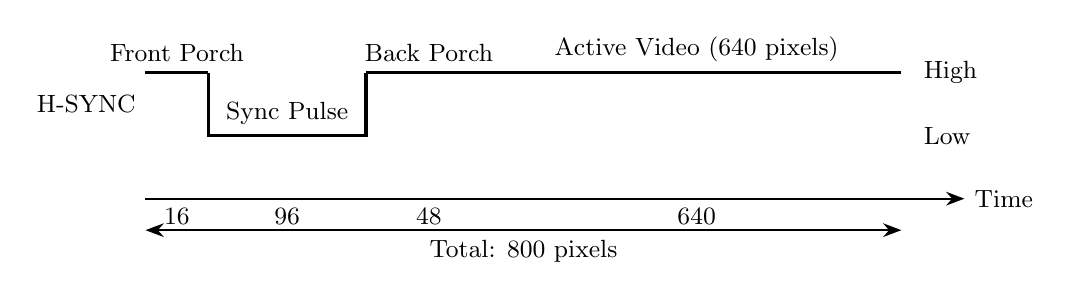
\begin{tikzpicture}[
    >=Stealth,
    scale=0.8,
    every node/.style={font=\small}
]

% Time axis
\draw[->, thick] (0,0) -- (13,0) node[right] {Time};

% H-SYNC signal
\draw[very thick] (0, 2) -- (1, 2) node[above, pos=0.5] {Front Porch};
\draw[very thick] (1, 2) -- (1, 1) -- (3.5, 1) node[above, pos=0.5] {Sync Pulse} -- (3.5, 2);
\draw[very thick] (3.5, 2) -- (5.5, 2) node[above, pos=0.5] {Back Porch};
\draw[very thick] (5.5, 2) -- (12, 2) node[above, pos=0.5] {Active Video (640 pixels)};

% Labels below
\node[below] at (0.5, 0) {16};
\node[below] at (2.25, 0) {96};
\node[below] at (4.5, 0) {48};
\node[below] at (8.75, 0) {640};

% Total
\draw[<->, thick] (0, -0.5) -- (12, -0.5) node[midway, below] {Total: 800 pixels};

% Signal label
\node[left] at (0, 1.5) {H-SYNC};

% High/Low labels
\node[right] at (12.2, 2) {High};
\node[right] at (12.2, 1) {Low};

\end{tikzpicture}
\caption{Horizontal Timing Diagram (640$\times$400 @ 70 Hz)}
\label{fig:htiming}
\end{figure}

\subsection{Vertical Timing}

The vertical timing waveform is shown in Figure~\ref{fig:vtiming}.

\begin{figure}[tbp]
\centering
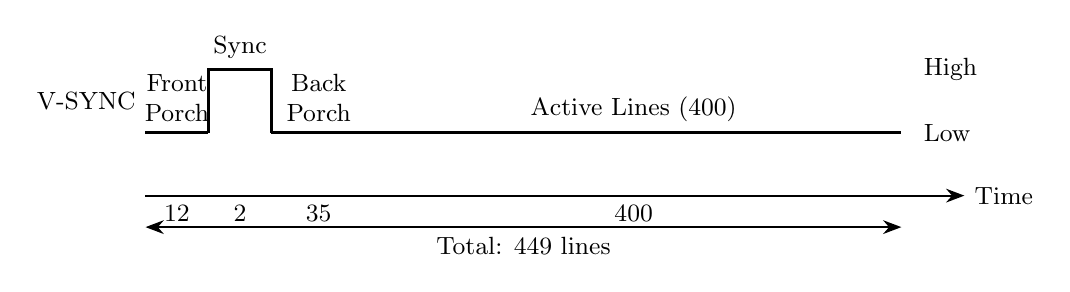
\begin{tikzpicture}[
    >=Stealth,
    scale=0.8,
    every node/.style={font=\small}
]

% Time axis
\draw[->, thick] (0,0) -- (13,0) node[right] {Time};

% V-SYNC signal (active high for 640x400)
\draw[very thick] (0, 1) -- (1, 1) node[above, pos=0.5, align=center] {Front\\Porch};
\draw[very thick] (1, 1) -- (1, 2) -- (2, 2) node[above, pos=0.5] {Sync} -- (2, 1);
\draw[very thick] (2, 1) -- (3.5, 1) node[above, pos=0.5, align=center] {Back\\Porch};
\draw[very thick] (3.5, 1) -- (12, 1) node[above, pos=0.5] {Active Lines (400)};

% Labels below
\node[below] at (0.5, 0) {12};
\node[below] at (1.5, 0) {2};
\node[below] at (2.75, 0) {35};
\node[below] at (7.75, 0) {400};

% Total
\draw[<->, thick] (0, -0.5) -- (12, -0.5) node[midway, below] {Total: 449 lines};

% Signal label
\node[left] at (0, 1.5) {V-SYNC};

% High/Low labels
\node[right] at (12.2, 2) {High};
\node[right] at (12.2, 1) {Low};

\end{tikzpicture}
\caption{Vertical Timing Diagram (640$\times$400 @ 70 Hz)}
\label{fig:vtiming}
\end{figure}

\section{File Manifest}

\begin{longtable}{ll}
\caption{VGA Controller File List}
\label{tab:file_list} \\
\toprule
\textbf{File} & \textbf{Purpose} \\
\midrule
\endfirsthead

\multicolumn{2}{c}{File Manifest -- continued} \\
\toprule
\textbf{File} & \textbf{Purpose} \\
\midrule
\endhead

\bottomrule
\endfoot

\bottomrule
\endlastfoot

\texttt{vga\_timing\_pkg.vhdl} & Timing constants and type definitions \\
\texttt{vga\_timing\_gen.vhdl} & VGA sync, blanking, and address generation \\
\texttt{framebuffer\_bram.vhdl} & Dual-port framebuffer BRAM (256 KB) \\
\texttt{palette\_bram.vhdl} & Dual-port palette RAM (256$\times$12-bit) \\
\texttt{axi\_slave.vhdl} & AXI4-Lite slave with burst and RMW support \\
\texttt{register\_bank.vhdl} & Control, buffer, and IRQ registers \\
\texttt{interrupt\_controller.vhdl} & Edge-detect and W1C interrupt logic \\
\texttt{generic\_register.vhdl} & Parameterised flip-flop register primitive \\
\texttt{vga\_framebuffer.vhdl} & Framebuffer + palette + register wrapper \\
\texttt{vga\_controller.vhdl} & Top-level integration \\
\texttt{vga\_controller\_tb\_comprehensive.vhdl} & Comprehensive simulation testbench \\
\texttt{vga\_controller.xdc} & Pin constraints (Nexys A7) \\
\texttt{create\_project.tcl} & Vivado project creation script \\
\texttt{README.md} & Quick reference guide \\
\end{longtable}

\section{Glossary}

\begin{description}
    \item[AXI] Advanced eXtensible Interface - ARM's standard for on-chip communication
    \item[BRAM] Block RAM - Dedicated memory blocks in FPGAs
    \item[Double-Buffering] Technique using two framebuffers to eliminate tearing
    \item[Frame Buffer] Memory holding pixel data for display
    \item[H-SYNC] Horizontal Synchronization pulse
    \item[Indexed Color] Color system using palette lookups
    \item[Palette] Lookup table mapping pixel indices to RGB colors
    \item[Pixel Clock] Clock rate at which pixels are output (25.175 MHz)
    \item[Tearing] Visual artifact from updating visible framebuffer
    \item[V-SYNC] Vertical Synchronization pulse
    \item[VGA] Video Graphics Array - Analog display standard
    \item[VHDL] VHSIC Hardware Description Language
\end{description}

\section{References}

\begin{enumerate}
    \item VESA Monitor Timing Specification
    \item Xilinx 7-Series FPGA Documentation
    \item AXI4-Lite Protocol Specification (ARM IHI 0022E)
    \item VGA Signal Specification
    \item Digilent Nexys A7 Reference Manual
\end{enumerate}

\section{Revision History}

\begin{table}[tbp]
\centering
\caption{Document Revision History}
\label{tab:revisions}
\begin{tabular}{lll}
\toprule
\textbf{Version} & \textbf{Date} & \textbf{Changes} \\
\midrule
1.0 & 2026-02-13 & Initial release \\
1.1 & 2026-02-20 & Updated base address to \texttt{0x48000000}; split Interrupt Control \\
    &            & into separate IRQ Enable (\texttt{0x40208}) and IRQ Clear/Status \\
    &            & (\texttt{0x4020C}) registers; corrected Buffer~1 start address to \\
    &            & \texttt{0x0FA00} (offset 64,000); corrected palette address range \\
    &            & to \texttt{0x40000--0x401FF}; updated file manifest \\
\bottomrule
\end{tabular}
\end{table}

\end{document}
